% Copyright 2021 Fausto Spoto
%
% Licensed under the Apache License, Version 2.0 (the "License");
% you may not use this file except in compliance with the License.
% You may obtain a copy of the License at
%
%    http://www.apache.org/licenses/LICENSE-2.0
%
% Unless required by applicable law or agreed to in writing, software
% distributed under the License is distributed on an "AS IS" BASIS,
% WITHOUT WARRANTIES OR CONDITIONS OF ANY KIND, either express or implied.
% See the License for the specific language governing permissions and
% limitations under the License.

\documentclass[11pt]{beamer}  %% versione proiettore
%%\documentclass[11pt,handout]{beamer} %% versione stampa
\usepackage{lucidiJb-2ed}
\usepackage{mathtools}
\usepackage[normalem]{ulem}

\usepackage{relsize}

\mode<article>
{
  \usepackage{fullpage}
  \usepackage{hyperref}
}

\mode<presentation>
{
  \setbeamertemplate{background canvas}[vertical shading][bottom=red!10,top=blue!10]
  \usetheme{Course}
  \usefonttheme[onlysmall]{structurebold}
}

\subtitle{Blockchain Course}
\title{Ethereum}
\institute{Universit\`a di Verona, Italy}
\date{February 2021}

\setbeamercovered{invisible}

\def\codesize{\smaller}
\def\<#1>{\codeid{#1}}
\newcommand{\codeid}[1]{\ifmmode{\mbox{\codesize\ttfamily{#1}}}\else{\codesize\ttfamily #1}\fi}

\begin{document}

\begin{frame}
  \titlepage
\end{frame}

\begin{frame}
  \frametitle{Thw world computer}

  \begin{greenbox}{}
    An open source, globally \alert{decentralized computing infrastructure}
    that executes programs called \alert{smart contracts}, written
    in a \alert{Turing-complete} programming language, translated into
    bytecode and run on a \alert{virtual machine}. It uses a
    \alert{blockchain} to synchronize and store the system's \alert{singleton state} changes
    (key/value tuples), along
    with a cryptocurrency called \alert{ether} to \alert{meter and constrain}
    execution resource costs. It enables developers to build
    \alert{decentralized applications} with \alert{built-in economic functions}
  \end{greenbox}

  \begin{center}
    
\includegraphics[scale=0.3,clip=false]{pictures/world-computer.jpg}
  \end{center}

\end{frame}

\begin{frame}\frametitle{DApps}

  \begin{greenbox}{DApps = smart contracts (Solidity) + web3 frontend (JavaScript\ldots)}
    \begin{center}
      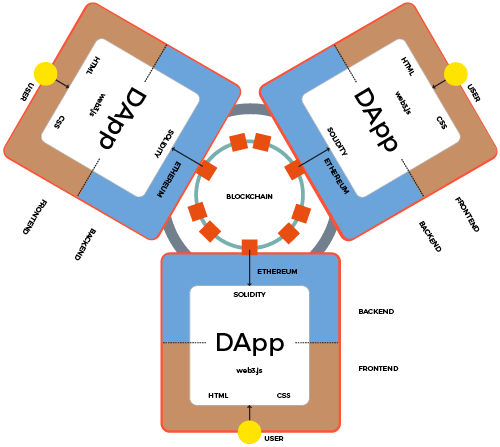
\includegraphics[scale=0.43,clip=false]{pictures/dapps.png}
    \end{center}
  \end{greenbox}

\end{frame}

\begin{frame}\frametitle{People behind Ethereum}

  \begin{center}
  \begin{tabular}{c@{\hskip 1.5cm}c}
    
\includegraphics[scale=.3,clip=false]{pictures/vitalik_buterin.jpg} &
    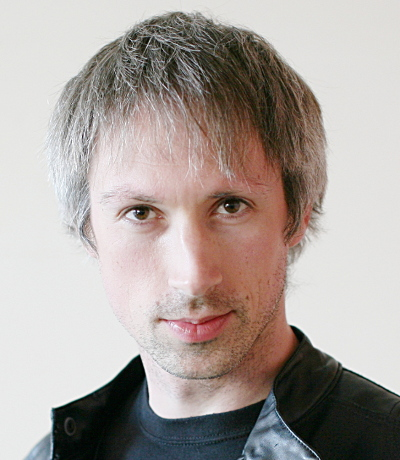
\includegraphics[scale=.247,clip=false]{pictures/gavin_wood.jpg} \\
    Vitalik Buterin & Gavin Wood
  \end{tabular}
  \end{center}
  
\end{frame}

\begin{frame}\frametitle{References used in this course}

  \begin{center}
    Yellow Paper: \url{https://ethereum.github.io/yellowpaper/paper.pdf}\\
    \mbox{}\\
    \begin{tabular}{c@{\hskip 1.5cm}c}
      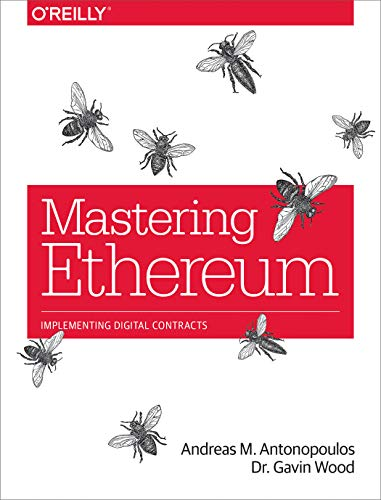
\includegraphics[scale=.3,clip=false]{pictures/mastering-ethereum.jpg} &
      
\includegraphics[scale=.3,clip=false]{pictures/building-games.jpg}
    \end{tabular}
  \end{center}

  \begin{center}
    The leftmost: \url{https://github.com/ethereumbook/ethereumbook}
  \end{center}

\end{frame}

\begin{frame}\frametitle{Deterministic (infinite) state machine}

  \begin{greenbox}{A very abstract view of blockchain}
    A blockchain is a distributed ledger of transaction requests, aggregated in blocks
    \begin{itemize}
    \item[] \hspace*{-3ex}\alert{Bitcoin:} transaction requests require a change of the set of UTXOs
    \item[] \hspace*{-3ex}\alert{Ethereum:} transaction requests require a change of a
      map $\mathit{key}\to\mathit{value}$
    \end{itemize}
    The change must be \alert{deterministic} otherwise consensus cannot be reached!
  \end{greenbox}

\end{frame}

\begin{frame}\frametitle{Ether denominations and unit names}

  \begin{center}
    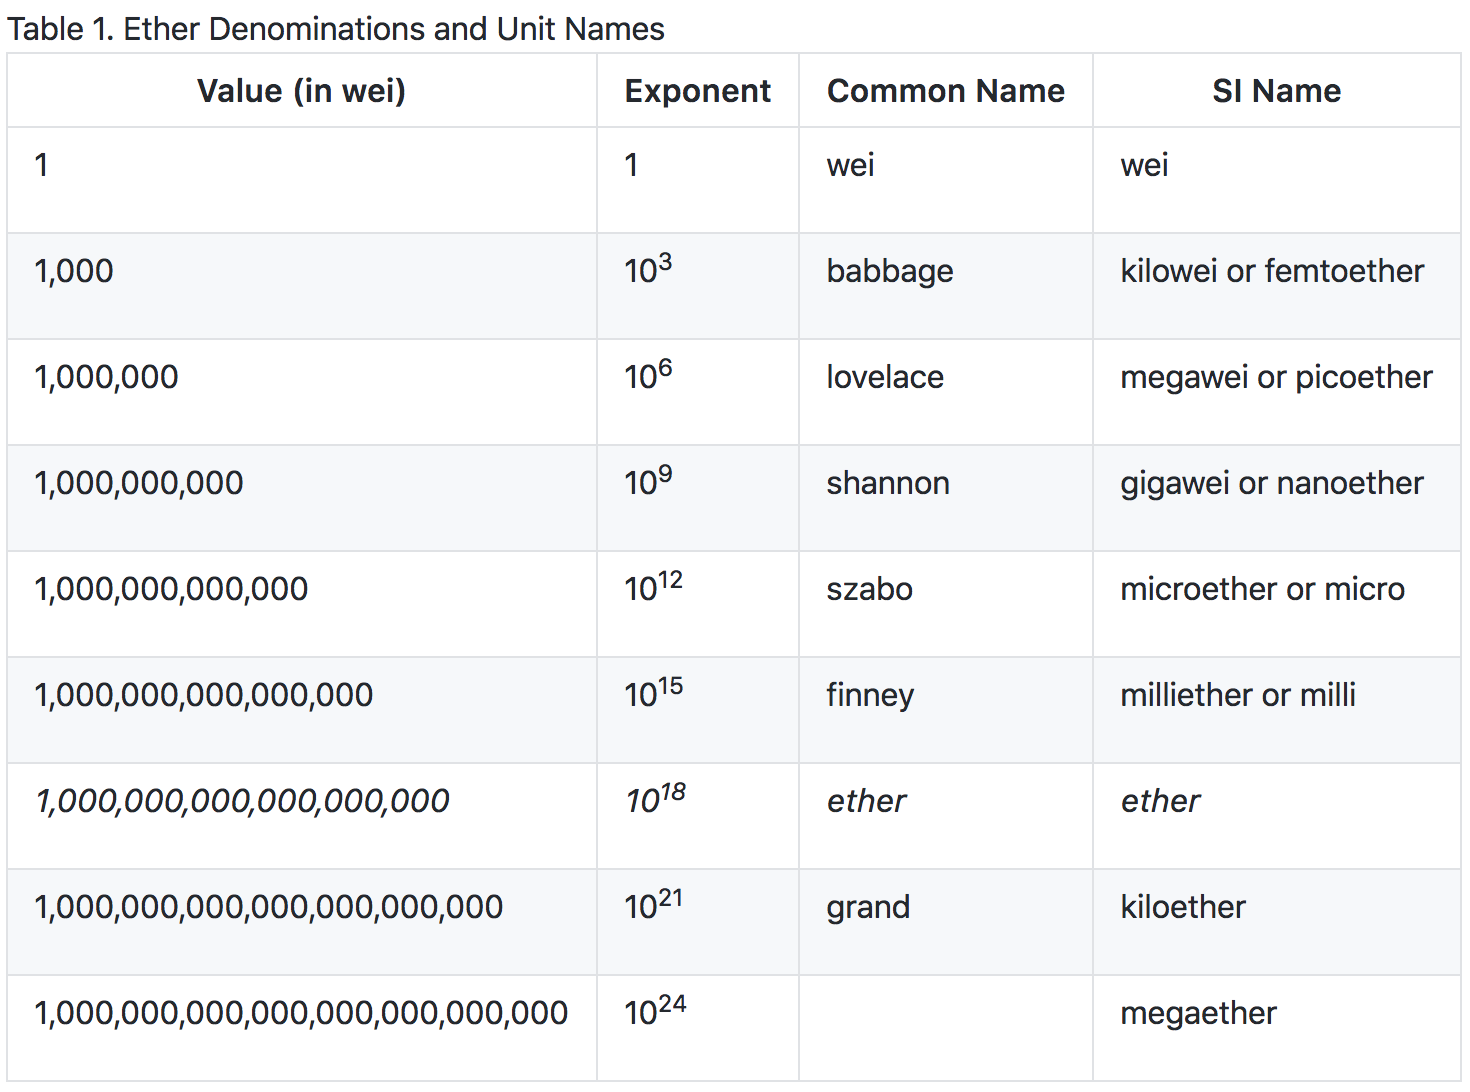
\includegraphics[scale=0.2,clip=false]{pictures/ether-denominations.png}
  \end{center}

\end{frame}

\begin{frame}\frametitle{Ether (ETH) price over the years}

  \begin{center}
    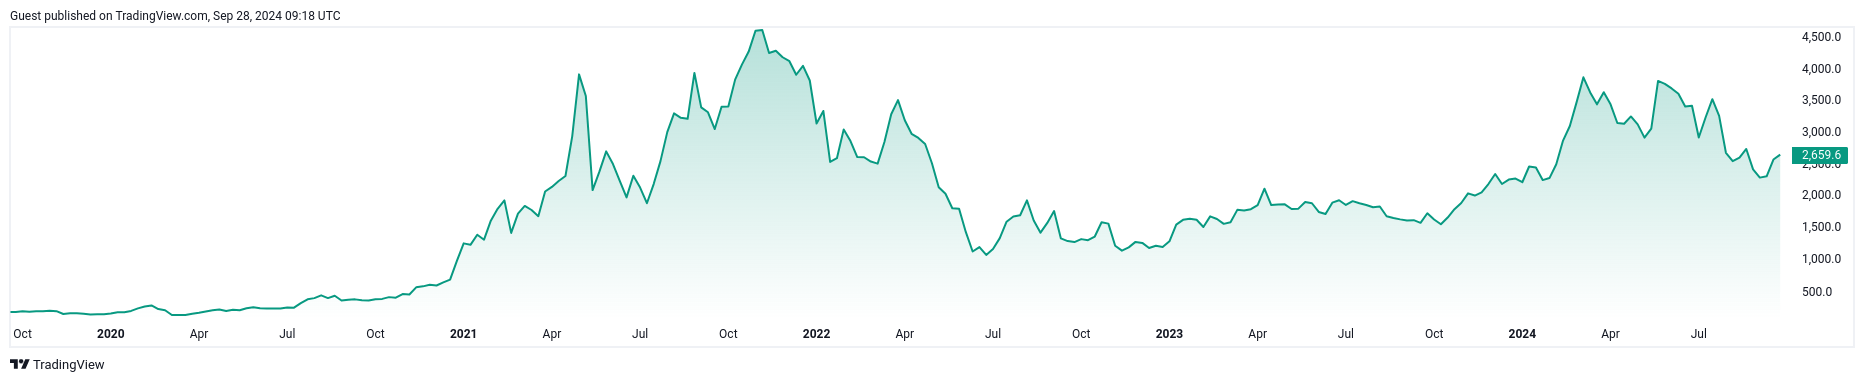
\includegraphics[scale=0.29,clip=false]{pictures/ether-chart.png}
  \end{center}

\end{frame}

\begin{frame}\frametitle{Ethereum Classic Ether (ETC) price over the years}

  \begin{center}
    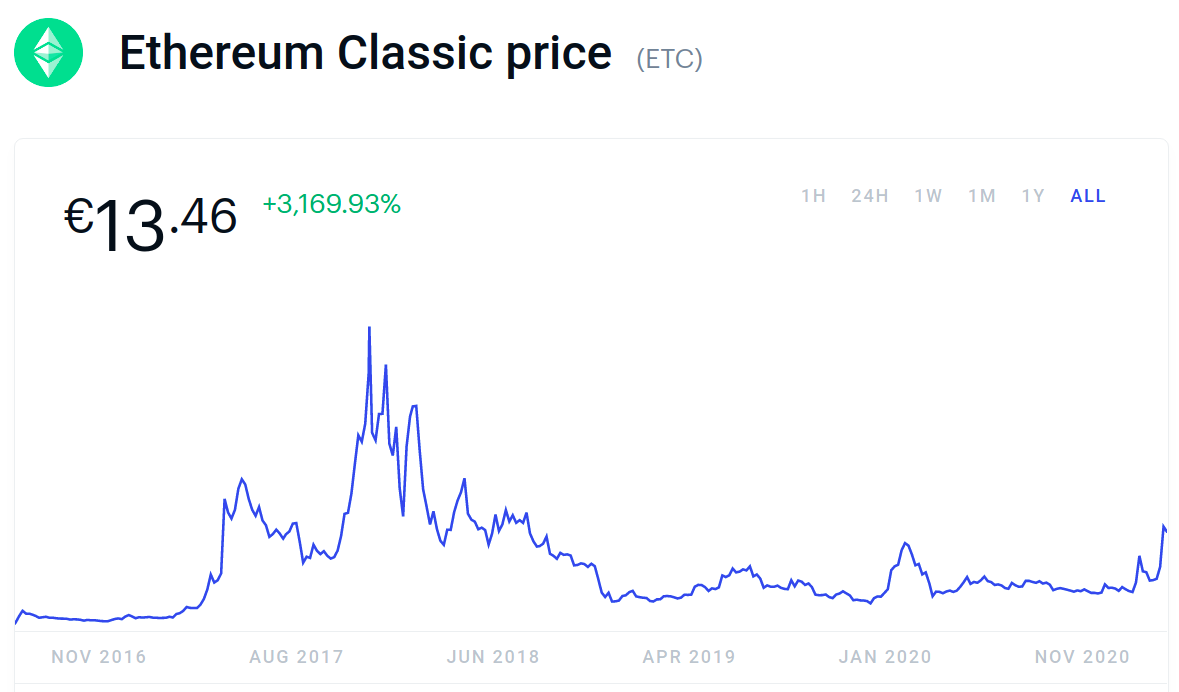
\includegraphics[scale=0.29,clip=false]{pictures/ether-classic-chart.png}
  \end{center}

\end{frame}

\begin{frame}\frametitle{Ethereum forks}

  \begin{center}
    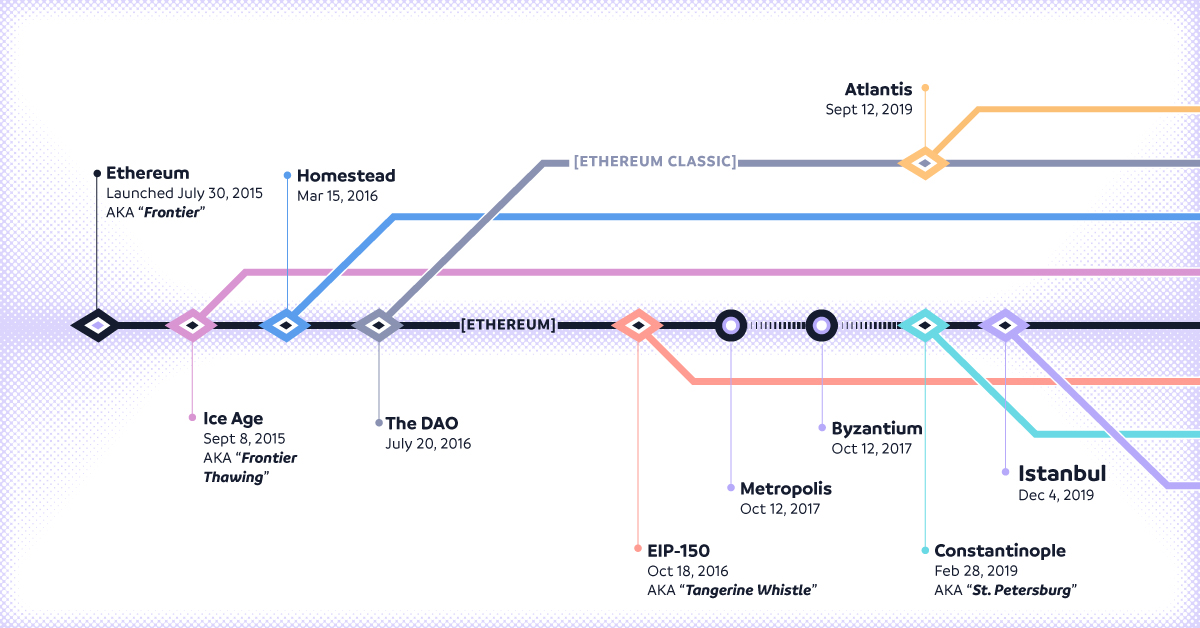
\includegraphics[width=\textwidth,clip=false]{pictures/ethereum-forks.jpg}
  \end{center}

\end{frame}

\begin{frame}\frametitle{Wallets}

  \begin{greenbox}{}
    A wallet is a
    software application that helps you manage your Ethereum account(s),
    by keeping your keys, creating and broadcasting transactions:
    \begin{itemize}
    \item mobile (Jaxx)
    \item desktop (Jaxx, Emerald Wallet)
    \item web-based (MetaMask, MyEtherWallet)
    \end{itemize}
  \end{greenbox}

\end{frame}

\begin{frame}\frametitle{MetaMask: create account}

  \url{https://metamask.io}
  \begin{center}
    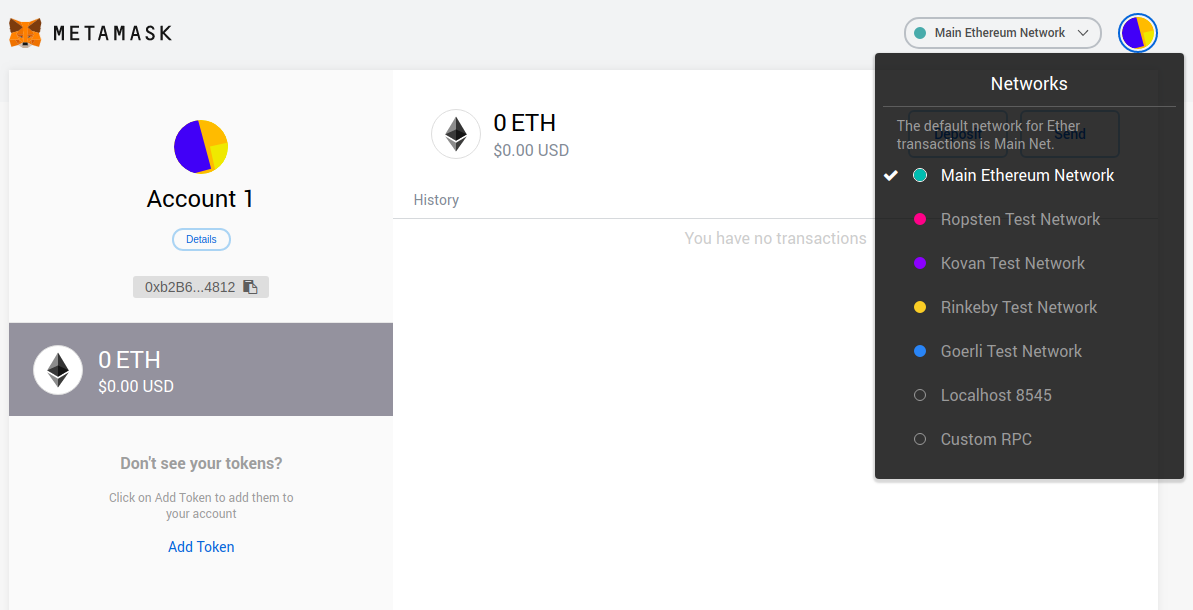
\includegraphics[width=\textwidth,clip=false]{pictures/metamask-account.png}
  \end{center}

\end{frame}

\begin{frame}\frametitle{MetaMask: connect to the faucet}

  \begin{center}
    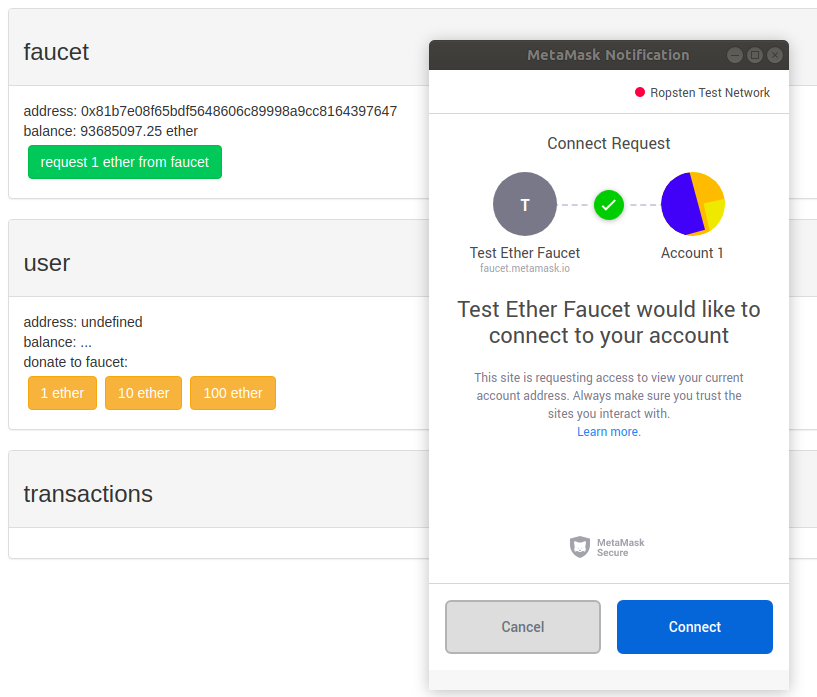
\includegraphics[scale=0.3,clip=false]{pictures/metamask-faucet.png}
  \end{center}

\end{frame}

\begin{frame}\frametitle{MetaMask: transaction for getting 1 ETH}

  \begin{center}
    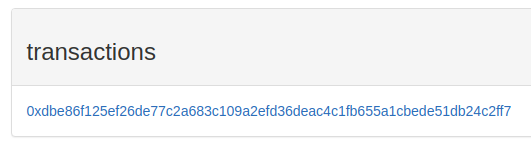
\includegraphics[width=\textwidth,clip=false]{pictures/metamask-faucet-transaction.png}
  \end{center}

\end{frame}

\begin{frame}\frametitle{MetaMask: detail of the transaction}

  \begin{center}
    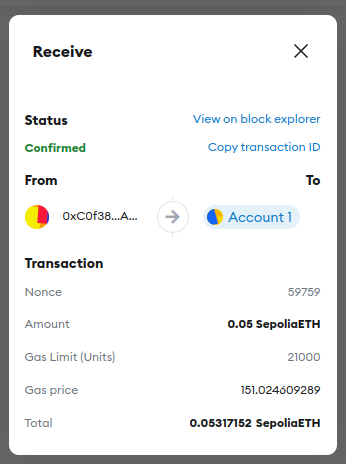
\includegraphics[scale=0.4,clip=false]{pictures/metamask-faucet-transaction-details.png}
  \end{center}

\end{frame}

\begin{frame}\frametitle{MetaMask: transactions of our account}

  \begin{center}
    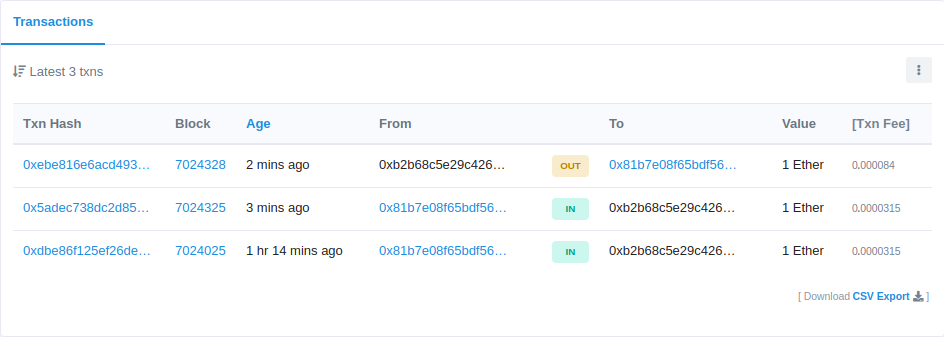
\includegraphics[width=\textwidth,clip=false]{pictures/metamask-faucet-transactions.png}
  \end{center}

\end{frame}

\begin{frame}\frametitle{Externally owned accounts (EOA) and contracts}

  \begin{greenbox}{}
    EOAs have keys, contracts have code, both have an address
  \end{greenbox}
  
  \begin{center}
    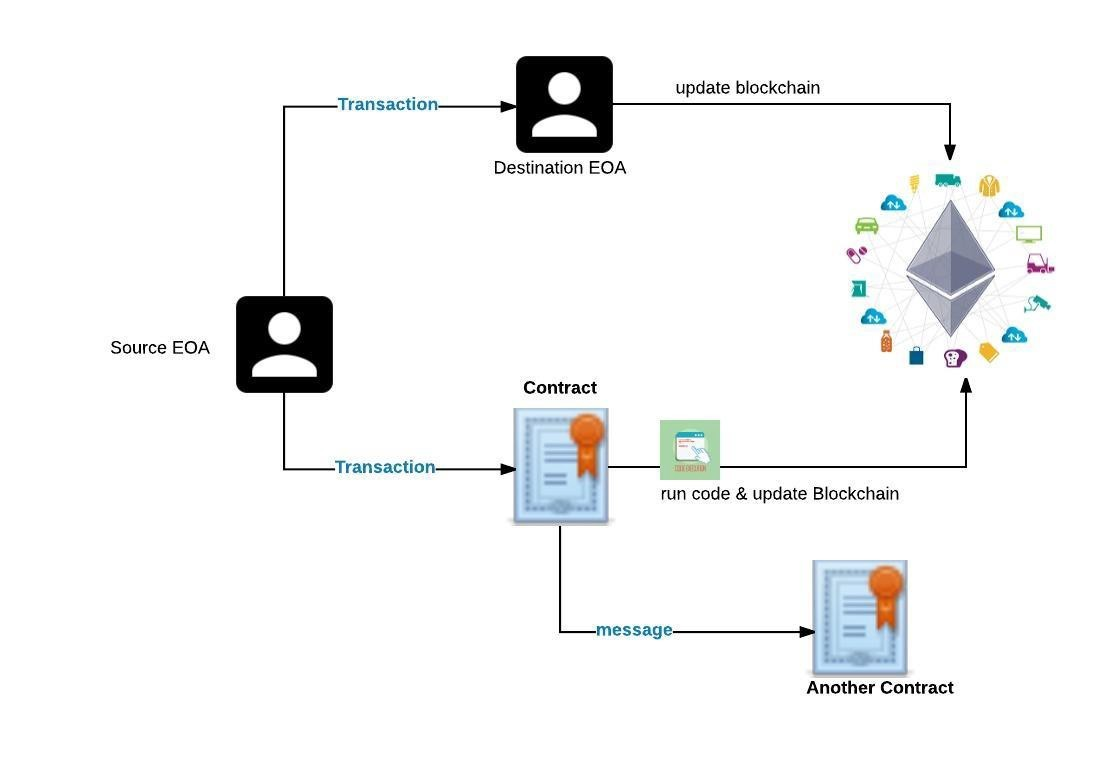
\includegraphics[scale=0.35,clip=false]{pictures/eoa-contract.jpg}
  \end{center}

\end{frame}

\begin{frame}\frametitle{A web IDE for Solidity: \url{https://remix.ethereum.org}}

  \begin{center}
    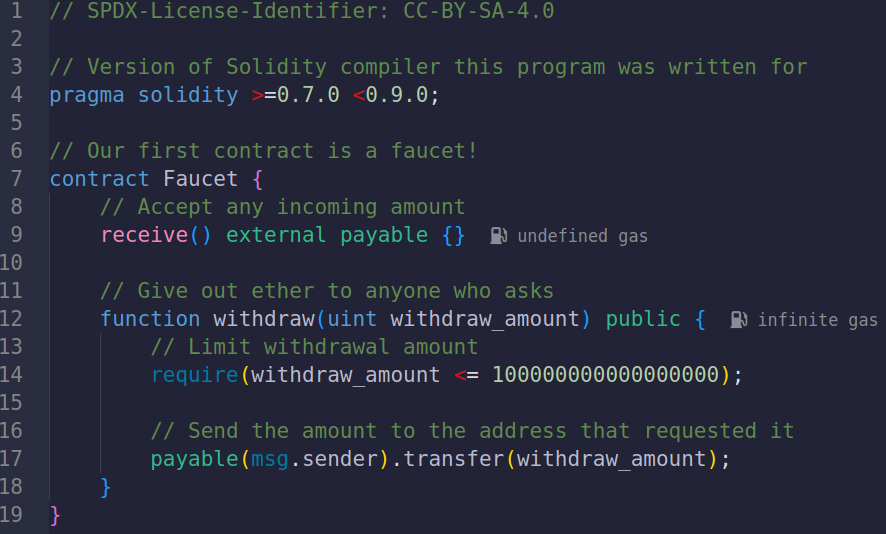
\includegraphics[scale=0.47,clip=false]{pictures/faucet_sol.png}
  \end{center}

\end{frame}

\begin{frame}\frametitle{Remix: deploy an instance of the contract}

  \begin{greenbox}{}
    Remix will create for us a transaction with the \<0x0> address as destination.
  \end{greenbox}

  \begin{center}
    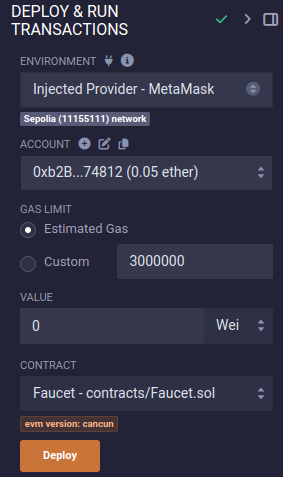
\includegraphics[scale=0.45,clip=false]{pictures/deploy-faucet.png}
  \end{center}

\end{frame}

\begin{frame}\frametitle{Remix: an instance of \<Faucet> has been deployed}

  \begin{center}
    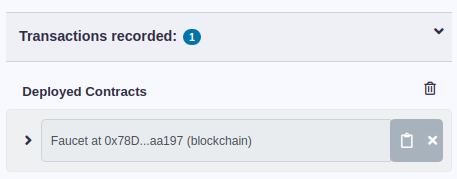
\includegraphics[scale=0.5,clip=false]{pictures/deployed-faucet.png}
  \end{center}

\end{frame}

\begin{frame}\frametitle{Check the outcome on Etherscan}

  \begin{greenbox}{}
    \url{https://ropsten.etherscan.io}
  \end{greenbox}

  \begin{center}
    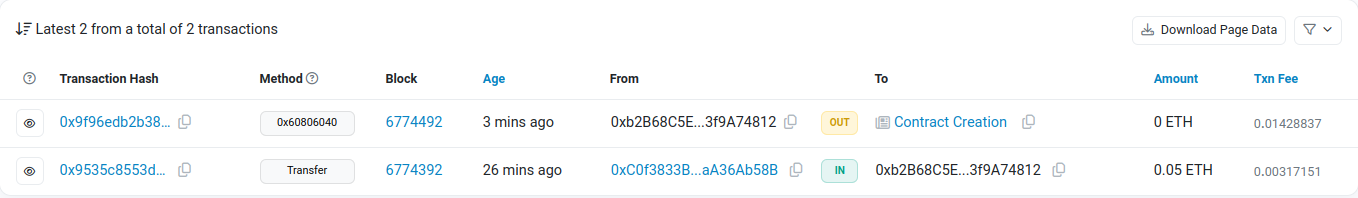
\includegraphics[width=\textwidth,clip=false]{pictures/faucet-etherscan.png}
  \end{center}

\end{frame}

\begin{frame}\frametitle{Send one Ether to the \<Faucet> through MetaMask}

  This corresponds to calling the default payable function.
  
  \begin{center}
    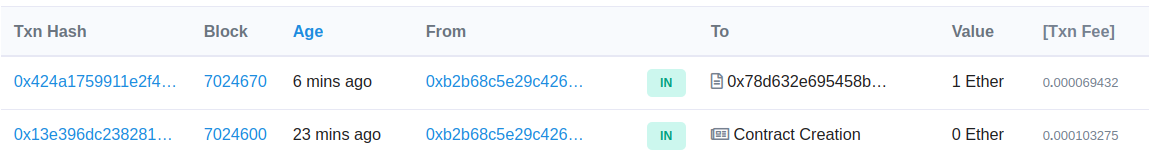
\includegraphics[width=\textwidth,clip=false]{pictures/faucet-etherscan2.png}
  \end{center}

\end{frame}

\begin{frame}\frametitle{Run the \<withdraw> function of the \<Faucet> in Remix}

  \begin{center}
    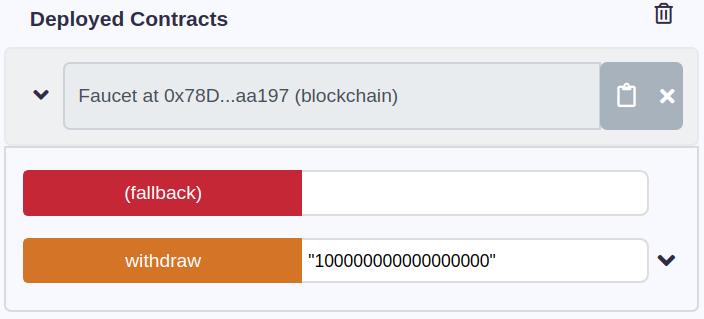
\includegraphics[width=\textwidth,clip=false]{pictures/faucet-withdraw.png}
  \end{center}

  \begin{center}
    $17$ zero's
  \end{center}
  
\end{frame}

\begin{frame}\frametitle{Check again on Etherscan}

  The faucet worked properly!
  
  \begin{center}
    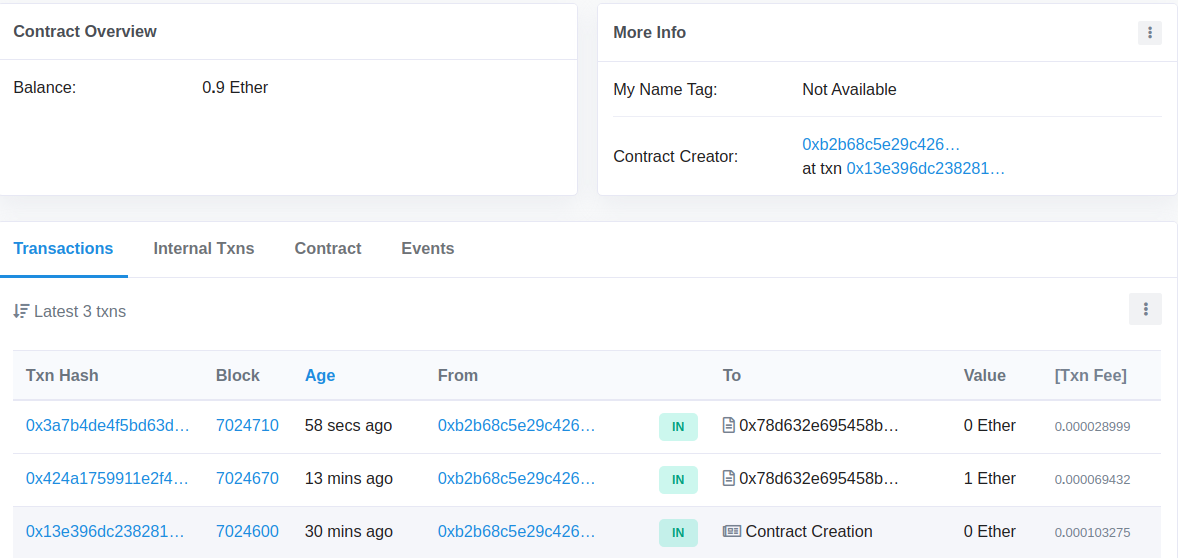
\includegraphics[width=\textwidth,clip=false]{pictures/faucet-etherscan3.png}
  \end{center}

\end{frame}

\begin{frame}\frametitle{The \<Faucet> has originated an internal transaction}

  \begin{center}
    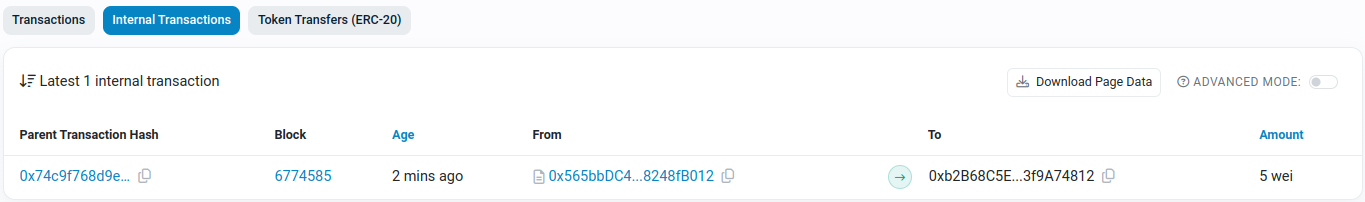
\includegraphics[width=\textwidth,clip=false]{pictures/faucet-etherscan-internal.png}
  \end{center}

  \begin{center}
    \<msg.sender.transfer(withdraw\_amount)>
  \end{center}

\end{frame}

\begin{frame}\frametitle{Ethereum clients}

  \begin{greenbox}{}
    An Ethereum client is a software application that implements
    the Ethereum specification (the \emph{Yellow Paper}) and communicates
    over the p2p network with other Ethereum clients
  \end{greenbox}

  \medskip

  \begin{itemize}
  \item Parity (Rust)
  \item Geth (Go)
  \item \<cpp-ethereum> (C++)
  \item \<pyethereum> (Python)
  \item Mantis (Scala)
  \item Harmony (Java)
  \end{itemize}

  \bigskip

  \begin{center}
    More clients means robustness against attacks
  \end{center}

\end{frame}

\begin{frame}\frametitle{Too big to fail?}

  \begin{center}
    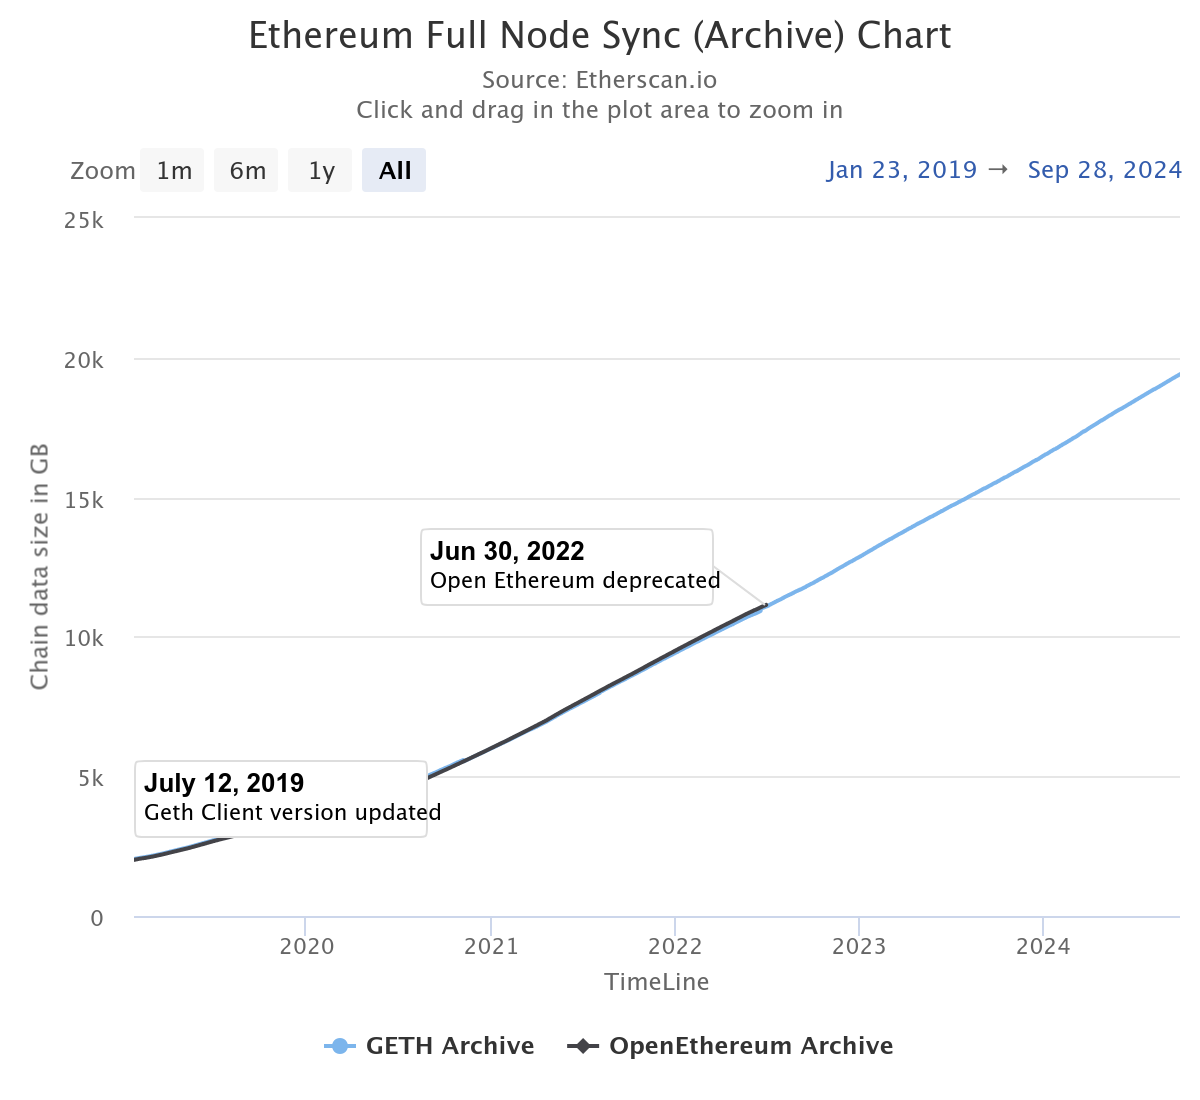
\includegraphics[scale=0.25,clip=false]{pictures/ethereum-size.png}
  \end{center}

  \begin{center}
    An 8TB SSD unit costs 160€ (2021)
  \end{center}

\end{frame}

\begin{frame}\frametitle{Client types}

  \begin{greenbox}{Full nodes}
    A full node stores the whole blockchain ($\sim$6TB) and
    takes part in mining. Very slow to synchronize.
    It can query the blockchain offline and
    without letting a third party know the information that it's reading
  \end{greenbox}

  \bigskip

  \begin{greenbox}{Remote clients}
    A remote client does not store the blockchain but
    depends on another full node for operation. They are wallets
    that create and broadcast transactions (for instance, MetaMask)
  \end{greenbox}

  \bigskip

  \begin{greenbox}{Networks}
    The \emph{mainnet}, or a \emph{testnet}, or a local blockchain (Ganache)
  \end{greenbox}
  
\end{frame}

\begin{frame}\frametitle{Infura: a cloud service to a full node}

  \url{https://infura.io}

  \begin{center}
    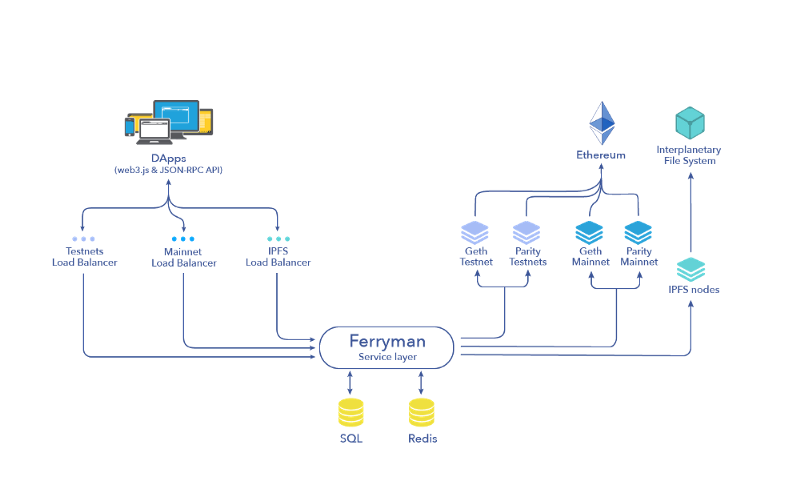
\includegraphics[width=\textwidth,clip=false]{pictures/infura.png}
  \end{center}

\end{frame}

\begin{frame}[fragile]\frametitle{Infura: ask for client version}

  \begin{greenbox}{}
    Register to Infura and create a project. Use the provided
    ID to build a query to Infura's JSON-RPC API:

\begin{semiverbatim}
$ \alert{curl https://mainnet.infura.io/v3/05550caa054f4fec80ff...
  -X POST
  -H "Content-Type: application/json"
  -d '\{"jsonrpc":"2.0","method":"web3_clientVersion",
  "params": [],"id":1\}'}
{\color{blue}\{"jsonrpc":"2.0","id":1,
  "result":"Geth/v1.9.25-omnibus-331c5f09
            /linux-amd64/go1.15.6"\}}
\end{semiverbatim}

\end{greenbox}

\end{frame}

\begin{frame}[fragile]\frametitle{Infura: ask for gas price}

  \begin{greenbox}{}
    Use your Infura ID to build a query to Infura's JSON-RPC API:

\begin{semiverbatim}
$ \alert{curl https://mainnet.infura.io/v3/05550caa054f4fec80ff...
  -X POST
  -H "Content-Type: application/json"
  -d '\{"jsonrpc":"2.0","method":"eth_gasPrice",
       "params": [],"id":1\}'}
{\color{blue}\{"jsonrpc":"2.0","id":1,"result":"{\color{black}0x248dede201}"\}}

$ \alert{echo $(({\color{black}0x248dede201}))}
{\color{blue}157000000001}
\end{semiverbatim}

  \end{greenbox}

\end{frame}

\begin{frame}\frametitle{Infura implements the Ethereum JSON-RPC API}

  \begin{center}
    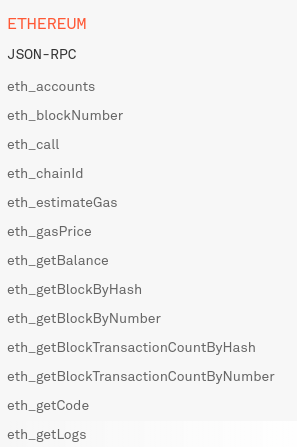
\includegraphics[scale=0.47,clip=false]{pictures/infura-json-rpc.png}
  \end{center}

\end{frame}

\begin{frame}[fragile]\frametitle{A Java client that connects to Infura}

  \begin{greenbox}{Import project \<ethereum-client> as an existing Maven project}
{\scriptsize\begin{alltt}
<project xmlns="http://maven.apache.org/POM/4.0.0"...>
  <modelVersion>4.0.0</modelVersion>
  {\color{violet}{<groupId>it.univr</groupId>
  <artifactId>it.univr.ethereumclient</artifactId>
  <version>0.0.1-SNAPSHOT</version>
  <name>Ethereum Client</name>}}
  {\color{red}{<build>
    <plugins><plugin>
        <groupId>org.apache.maven.plugins</groupId>
        <artifactId>maven-compiler-plugin</artifactId>
        <version>3.8.1</version>
        <configuration><release>11</release></configuration>
    </plugin></plugins>
  </build>}}
  {\color{blue}{<dependencies>
    <dependency>
      <groupId>org.web3j</groupId>
      <artifactId>core</artifactId>
      <version>5.0.0</version>
    </dependency>
  </dependencies>}}
</project>
\end{alltt}}
  \end{greenbox}
\end{frame}

\begin{frame}\frametitle{A Java client that connects to Infura}

  \begin{center}
    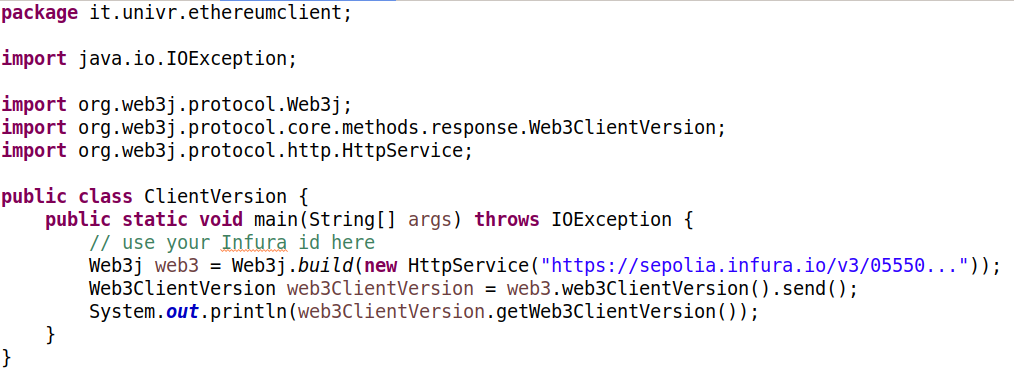
\includegraphics[width=\textwidth,clip=false]{pictures/client-version-java.png}
  \end{center}

  \bigskip

  \begin{center}
    \url{https://javadoc.io/doc/org.web3j}
  \end{center}

\end{frame}

\begin{frame}\frametitle{Ethereum's cryptographic hash function}

  \begin{greenbox}{Keccak-256}
    Ethereum uses the Keccak-256 cryptographic hash function.
    It is the original algorithm that won the SHA-3 Cryptographic Hash
    Function Competition of 2007. NIST standardized it in a slightly
    modified way as SHA-3. However, the Ethereum team never trusted
    such modification and used the original algorithm
  \end{greenbox}

  \bigskip

  \begin{redbox}{Keccak-256 or SHA-3?}
    You can still see blogs and even the source code of Ethereum refer
    to SHA-3. Despite of that, \underline{Etherem does not use SHA-3}, but the original
    Keccak-256 algorithm!
  \end{redbox}

\end{frame}

\begin{frame}\frametitle{Derivation of an Ethereum address from the private key}

  \begin{greenbox}{}
    Compute the public key,
    hash it with Keccak-256, keep only the last $20$ bytes (\emph{ie.}, $160$ bits, that is, $40$ hex digits). No checksum!
  \end{greenbox}
  
  \begin{center}
    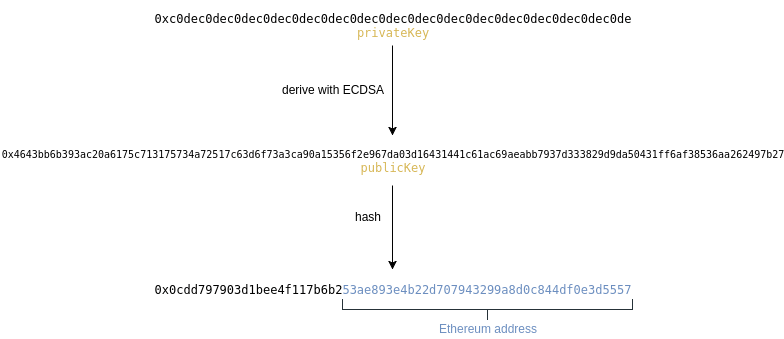
\includegraphics[width=\textwidth,clip=false]{pictures/ethereum-address-derivation.png}
  \end{center}

  \begin{center}
    \begin{itemize}
    \item[] {\color{red}Bitcoin:} private $\xRightarrow{\mathit{ECDSA}}$ public
      $\xRightarrow{\mathit{sha256}}$
      hash $\xRightarrow{\mathit{ripemd160}}$ address
    \item[] {\color{red}Ethereum:} private $\xRightarrow{\mathit{ECDSA}}$ public
      $\xRightarrow{\mathit{kekkak256}}$
      hash $\xRightarrow{\mathit{last\ 20\ bytes}}$ address
    \end{itemize}
  \end{center}

\end{frame}

\begin{frame}\frametitle{Checksummed address format: ICAP}

  \begin{greenbox}{}
    \<XE> + 2 characters of checksum + base-36 integer of up to 30 digits
  \end{greenbox}

  \bigskip

  \begin{greenbox}{}
    \begin{itemize}
    \item the base-36 integer can represent up to 155 bits, hence ICAP
      can only be used for addresses starting with a zero byte
    \item ICAP is compatible with IBAN
    \end{itemize}
  \end{greenbox}

  \bigskip

  \begin{greenbox}{Example}
    Ethereum address: \<0x001d3f1ef827552ae1114027bd3ecf1f086ba0f9>
    
    ICAP: \<XE60 HAMI CDXS V5QX VJA7 TJW4 7Q9C HWKJ D>
  \end{greenbox}

\end{frame}

\begin{frame}[fragile]\frametitle{Hex encoding with checksum in capitalization (EIP-55)}

  \begin{greenbox}{A backward compatible checksum injection}
    \begin{enumerate}
    \item use Keccak-256 to compute $64$ hex digits from the uncapitalized $40$ hex digits of the Ethereum address
    \item capitalize each alphabetic address character if the corresponding hex digit
      of the hash is greater than or equal to \<0x8>
    \end{enumerate}
  \end{greenbox}

  \bigskip

  \begin{greenbox}{Example}
\begin{semiverbatim}
Address:   001d3{\color{purple}f}1ef827552{\color{purple}a}e1114027{\color{purple}bd}3{\color{purple}ecf}1f086b{\color{purple}a}0{\color{purple}f}9
Keccak256: 23a69{\color{blue}c}1653e4ebb{\color{blue}b}619b0b2c{\color{blue}b8}a{\color{blue}9ba}d49892{\color{blue}a}8{\color{blue}b}9...
Result:    001d3{\color{red}F}1ef827552{\color{red}A}e1114027{\color{red}BD}3{\color{red}ECF}1f086b{\color{red}A}0{\color{red}F}9
\end{semiverbatim}
  \end{greenbox}

  \bigskip

  \begin{greenbox}{Checking procedure of an EIP-55 encoded address}
    \begin{itemize}
    \item apply the above capitalization procedure to it
    \item the result must match the EIP-55 encoded address
    \end{itemize}
  \end{greenbox}

\end{frame}

\begin{frame}\frametitle{Ethereum transactions}

  \begin{greenbox}{}
    A transaction is a signed message originated by an EOA, transmitted
    by the Ethereum network, and recorded on the Ethereum blockchain:
    \begin{itemize}
    \item nonce: sequence number per each originating EOA
    \item gas price: maximum willing to pay
    \item gas limit: maximum willing to consume
    \item to: recipient (destination address)
    \item value: ether sent to destination
    \item data: generic payload (method name, parameters, contract code\ldots)
    \item v,r,s: ECDSA signature of the originating EOA
    \end{itemize}
  \end{greenbox}

  \begin{center}
    The address of the originating EOA is implied by v,r,s\\
    The id of the transaction is the hash of its byte encoding
  \end{center}

\end{frame}

\begin{frame}\frametitle{Many kinds of transactions}

  \begin{center}
    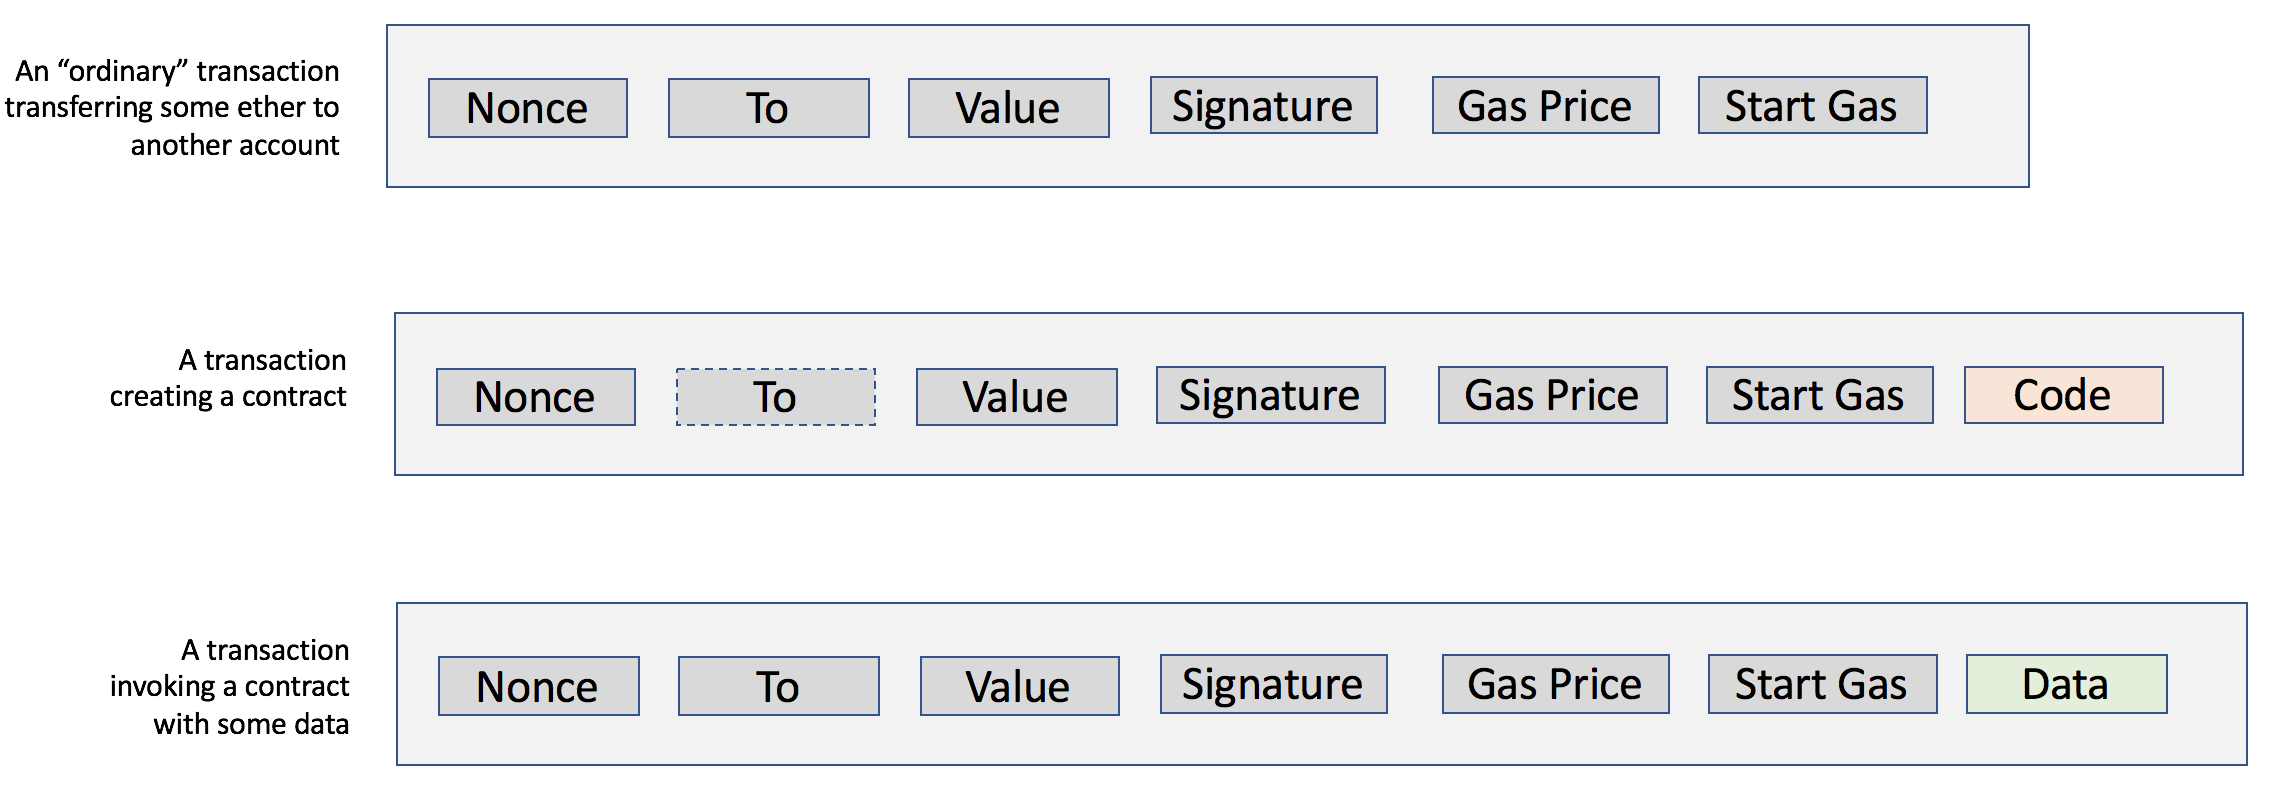
\includegraphics[width=\textwidth,clip=false]{pictures/many-transactions.png}
  \end{center}

\end{frame}

\begin{frame}\frametitle{Transaction lifecycle}

  \begin{center}
    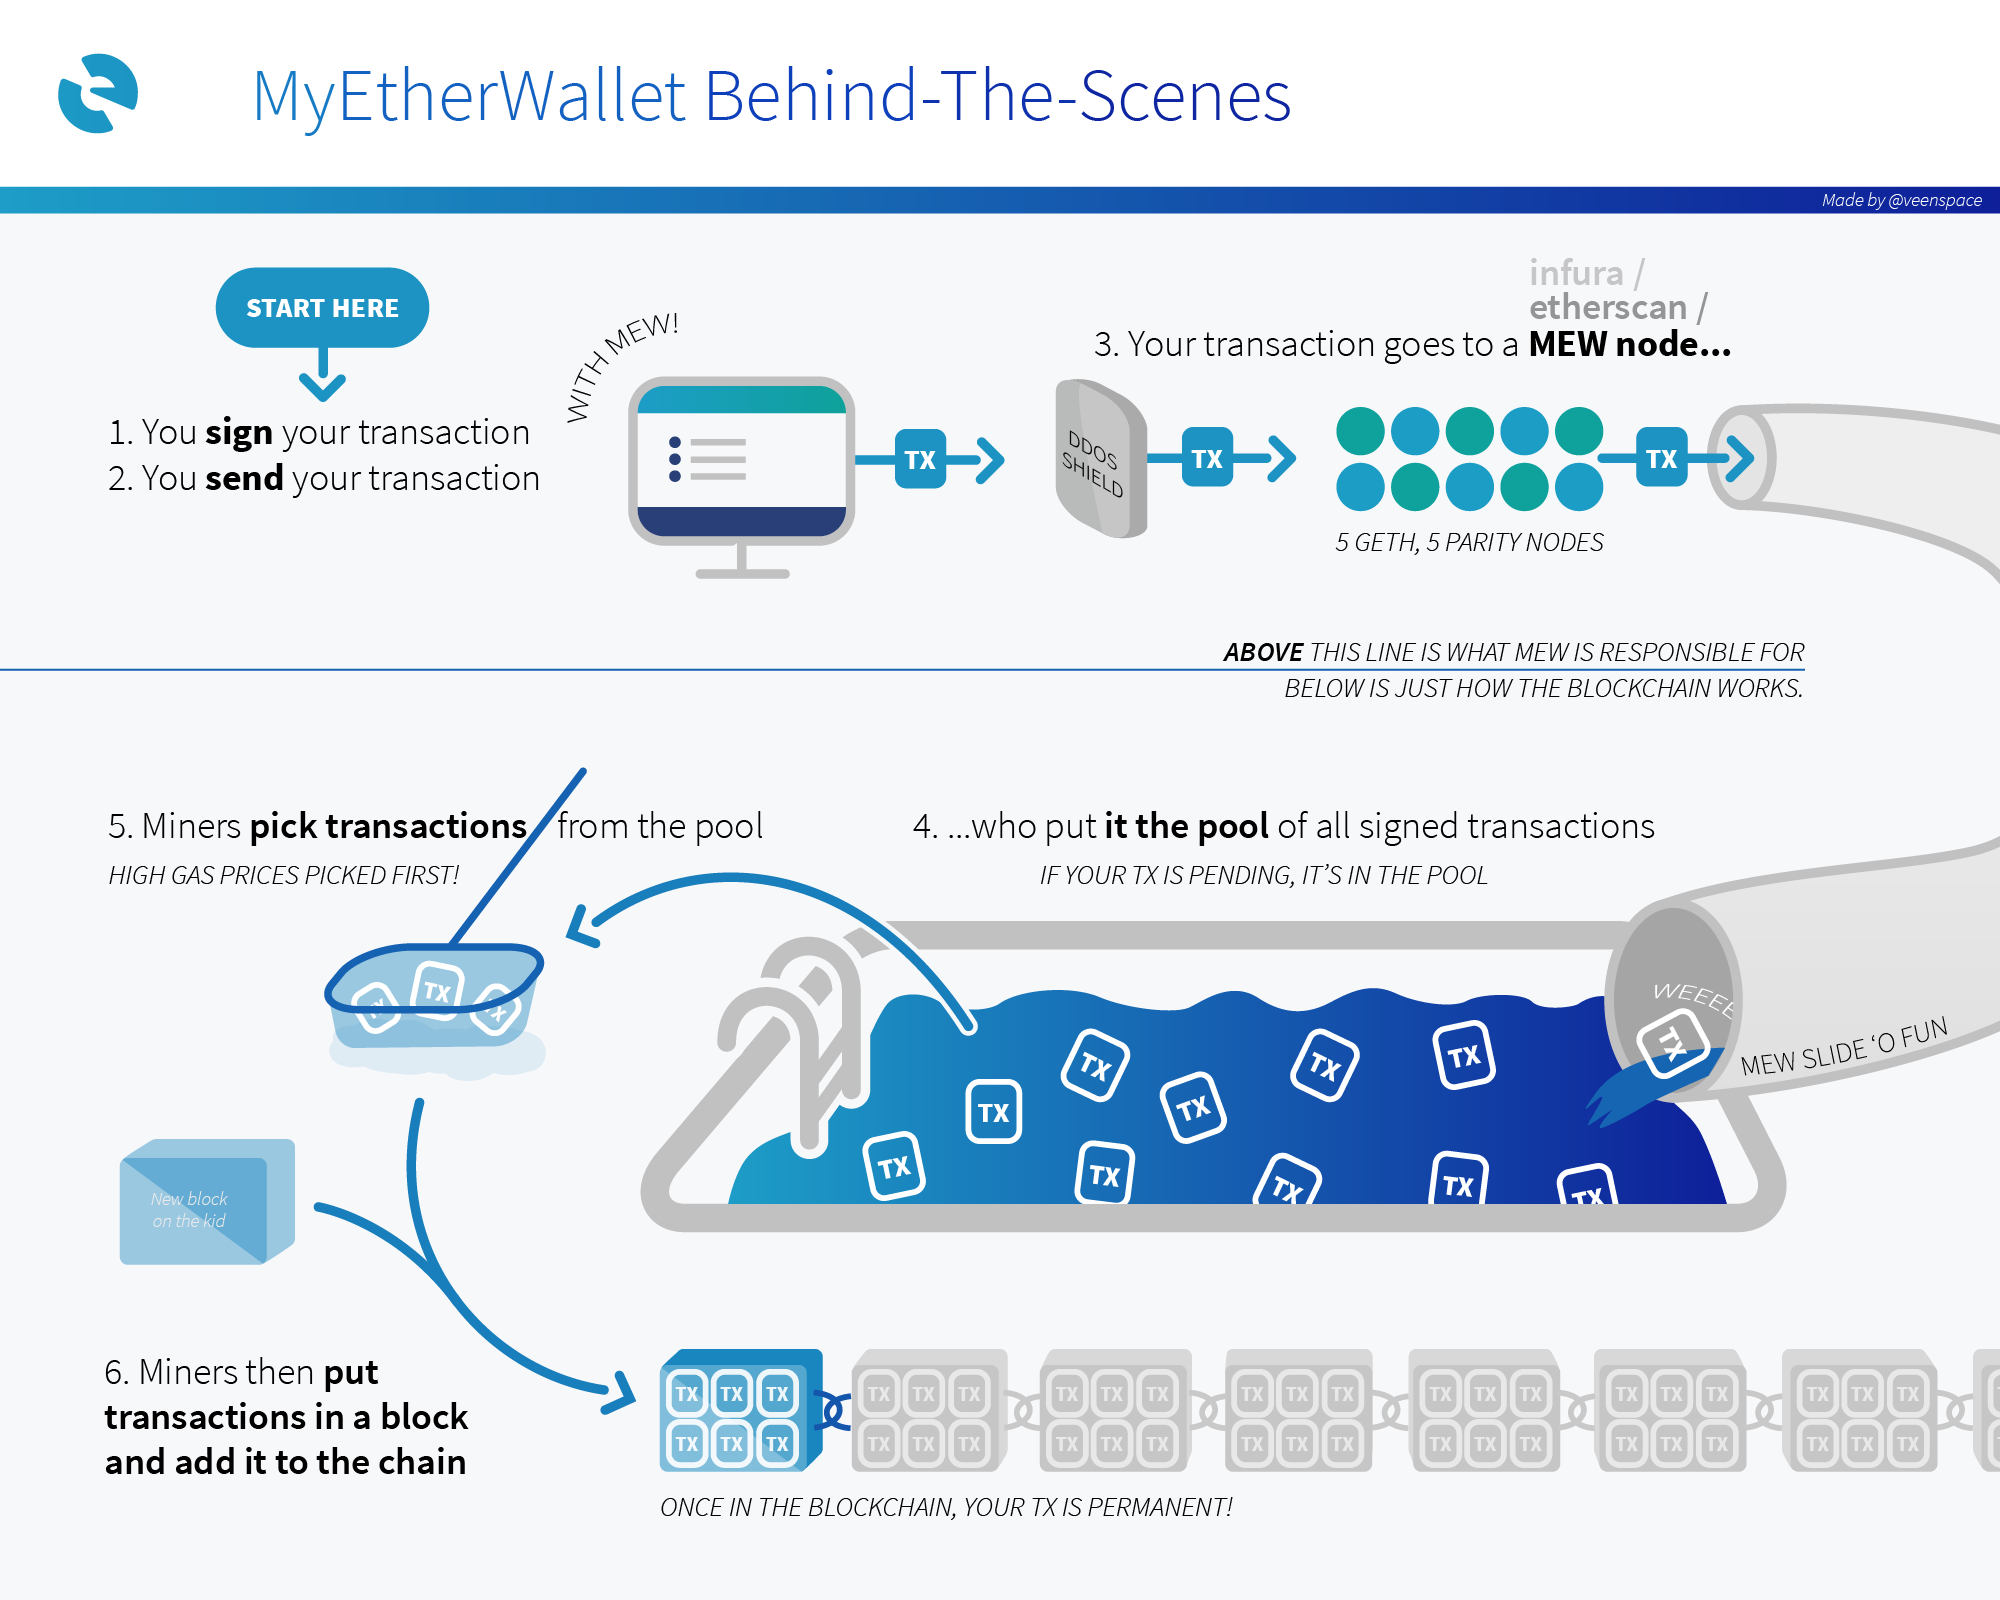
\includegraphics[scale=0.135,clip=false]{pictures/ethereum-transaction-life.png}
  \end{center}

\end{frame}

\begin{frame}\frametitle{Transactions induce state transitions}

  \begin{center}
    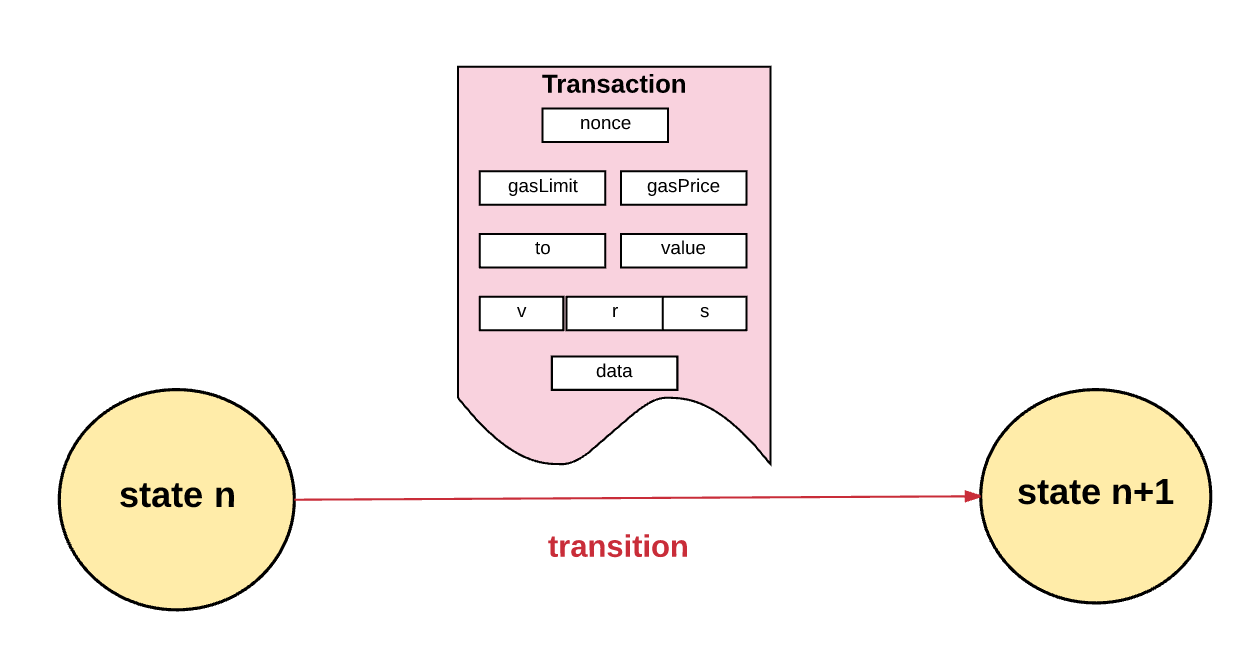
\includegraphics[width=\textwidth,clip=false]{pictures/state-transition.png}
  \end{center}

\end{frame}

\begin{frame}\frametitle{The nonce}

  \begin{greenbox}{The nonce of an EOA}
    A scalar value equal to the number of transactions sent from the EOA
  \end{greenbox}

  \bigskip

  \begin{greenbox}{Wallets keep track of nonces}
    They increase it and attach to each transaction they create per
    originating EOA
  \end{greenbox}

  \bigskip

  \begin{greenbox}{Nodes check nonces}
    They count the number $n$ of transactions originated
    by the EOA. If the nonce is smaller than $n+1$, the
    transaction is rejected. If the nonce is greater than $n+1$,
    the transaction is delayed and not yet executed:
    \begin{itemize}
    \item this guarantees transaction ordering
    \item and avoids transaction replaying
    \end{itemize}
  \end{greenbox}

  \bigskip

  \begin{redbox}{}
    \begin{center}
      Keeping track of nonces is hard for concurrent clients!
    \end{center}
  \end{redbox}

\end{frame}

\begin{frame}\frametitle{Why Bitcoin's transactions have no nonce?}

  \begin{greenbox}{Bitcoin's transactions can only transform UTXOs into TXOs}
    It is not possible to spend a UTXO again, inside the same history:
    it would be against the consensus rules
    \begin{itemize}
    \item[$\Rightarrow$] Executing a valid transaction today makes it invalid tomorrow
    \end{itemize}
  \end{greenbox}

  \bigskip

  \begin{greenbox}{Ethereum's transactions can induce any state change or fail}
    A valid (syntactically correct) transaction can always be executed in Ethereum
    \begin{itemize}
    \item[$\Rightarrow$] Executing a valid transaction today doesn't make it invalid tomorrow
      \alert{(without a nonce)}
    \end{itemize}
  \end{greenbox}

\end{frame}

\begin{frame}\frametitle{Computing the next nonce in Java using Infura}

  \begin{center}
    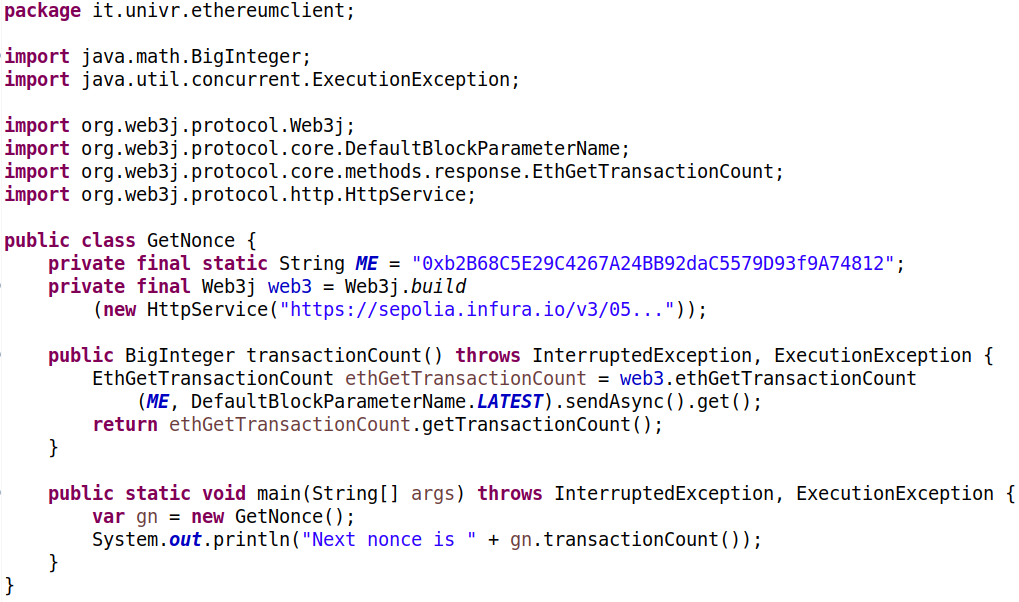
\includegraphics[width=\textwidth,clip=false]{pictures/get-nonce-java.png}
  \end{center}

\end{frame}

\begin{frame}\frametitle{Gas}

  The price of gas fluctuates, for protection against ETH spikes:

  \medskip

  \begin{greenbox}{\url{https://ethgasstation.info/}}
    \begin{center}
      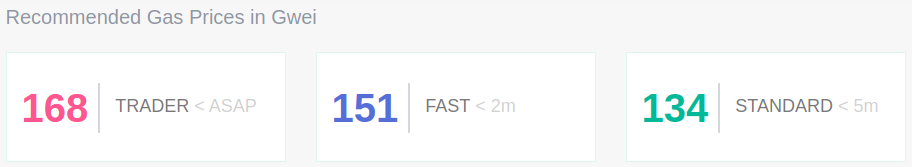
\includegraphics[width=\textwidth,clip=false]{pictures/ethgasstation.png}
    \end{center}
  \end{greenbox}

  \bigskip

  It is theoretically possible that transactions with $0$ gas price will be eventually
  processed

  \medskip

  Maximal fees: $\mathit{Gas\ price}\times\mathit{Gas\ limit}
  \times \mathit{Euros\ per\ Gwei}$

  \medskip

  \begin{redbox}{Example: a small transaction requires 21000 units of gas}
    \begin{center}
      $\mathit{fees} = 151\times 21000\times 0.00000162$€$=5.137$€
    \end{center}
  \end{redbox}
  
\end{frame}

\begin{frame}\frametitle{Average fees chart}

  \begin{greenbox}{\url{https://blockchair.com/}}
    \begin{center}
      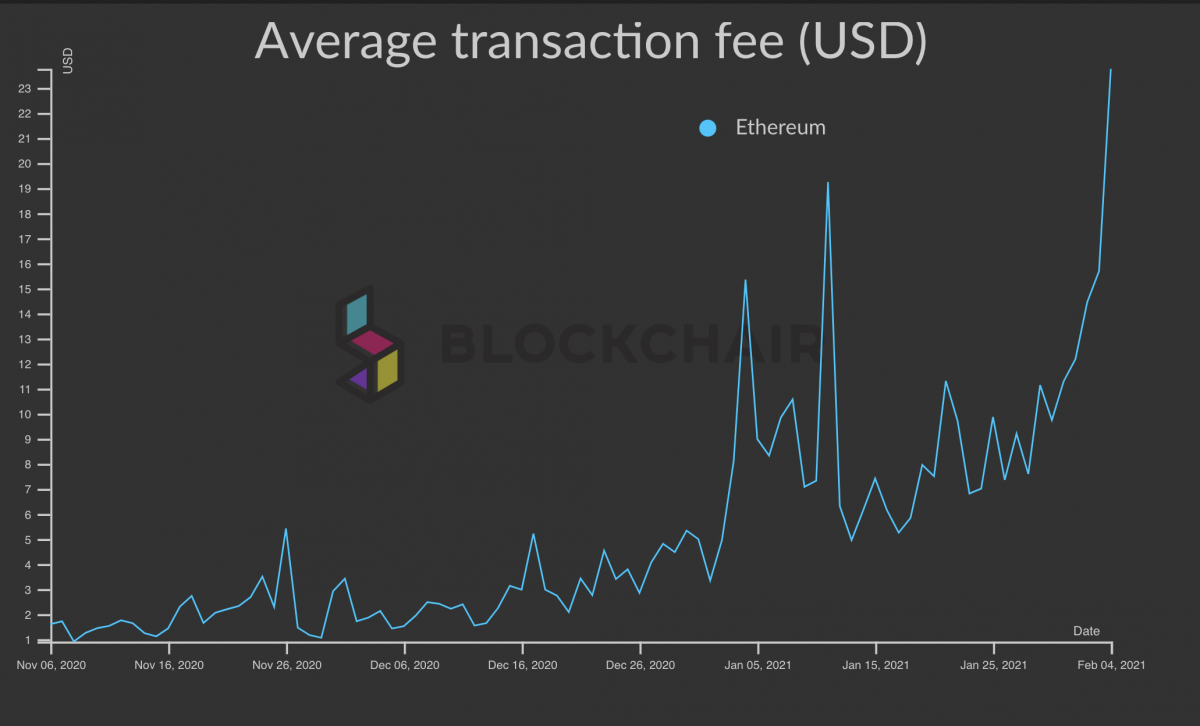
\includegraphics[width=\textwidth,clip=false]{pictures/ethereum-fees-chart.png}
    \end{center}
  \end{greenbox}

\end{frame}

\begin{frame}\frametitle{Computing the gas price in Java using Infura}

  \begin{center}
    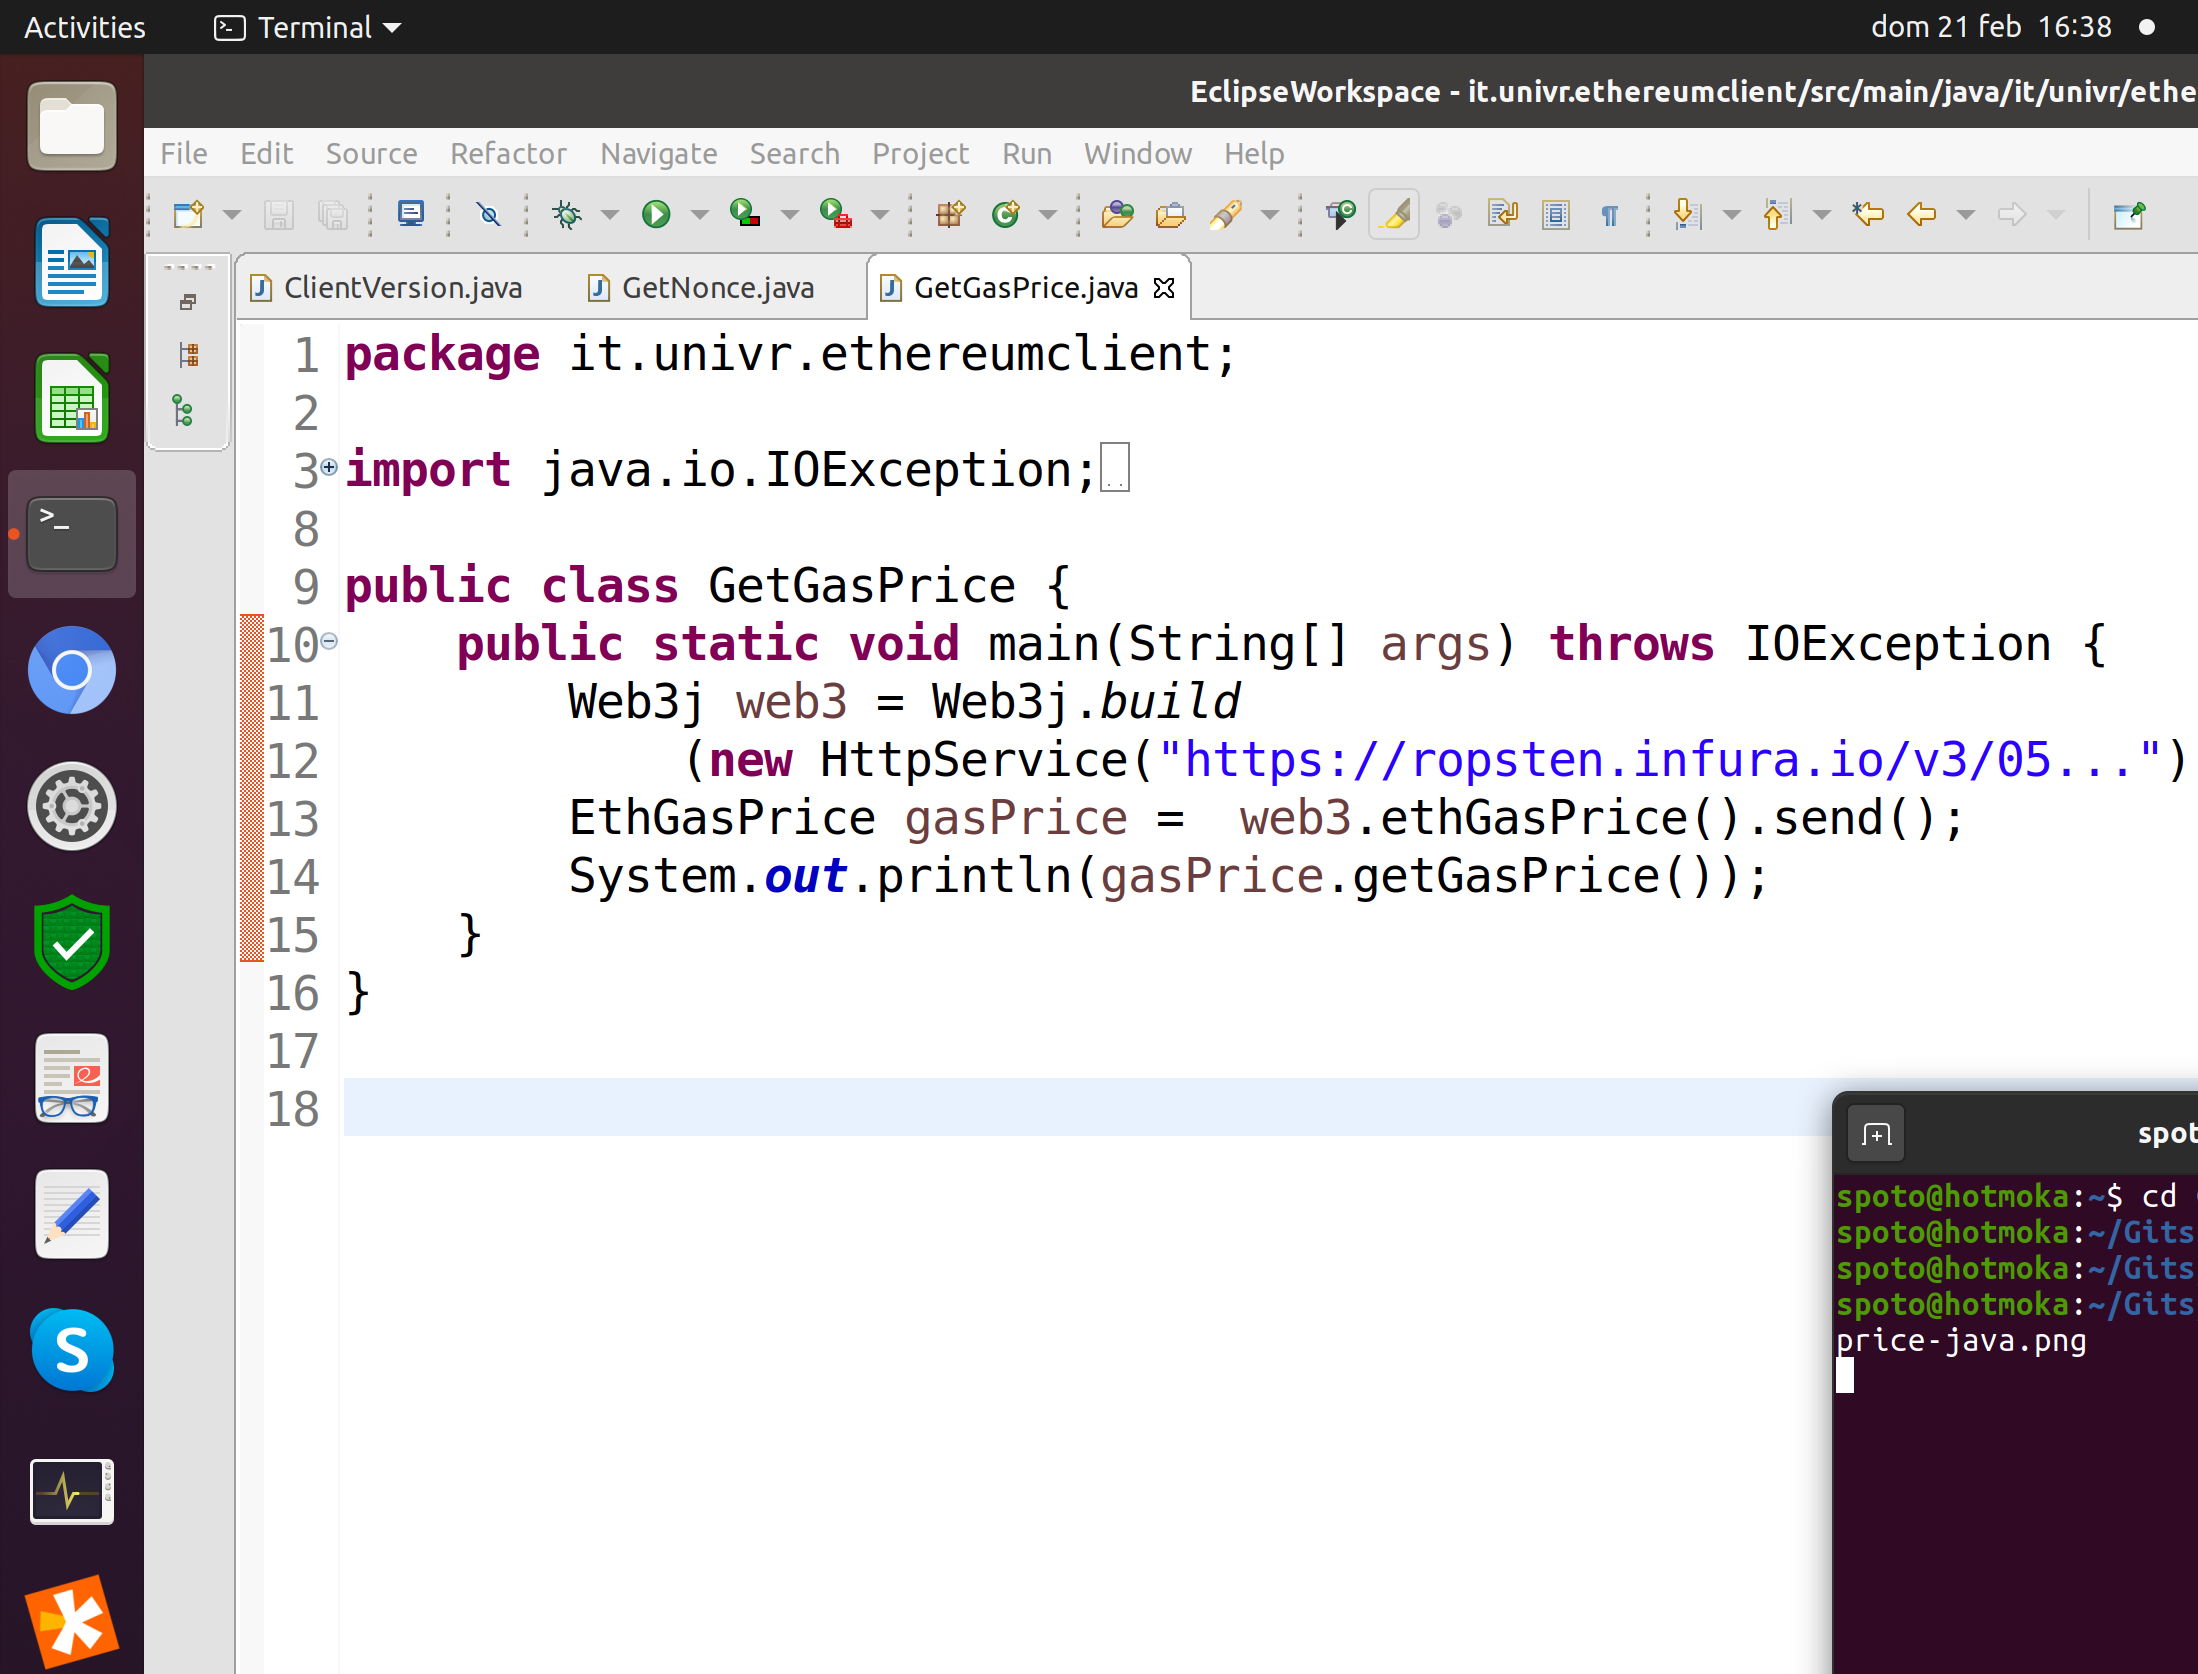
\includegraphics[width=\textwidth,clip=false]{pictures/get-gas-price-java.png}
  \end{center}

\end{frame}

\begin{frame}\frametitle{To}

  Any $20$ bytes recipient address can be specified (EOA or contract),
  there is no control!

  \bigskip

  \begin{redbox}{Burning ETH}
    Sending ether to a nonexistent address means \emph{burning} that ether,
    since it's practically impossible to identify the private key
    that controls that address. It is standard practice to burn ether
    by sending it to the address
    \begin{center}
      \<0x000000000000000000000000000000000000dEaD>
    \end{center}
  \end{redbox}

  \bigskip

  Clients should check for correctness of addresses, for instance
  through EIP-55
\end{frame}

\begin{frame}\frametitle{Signing and sending a transaction in Java}

  \begin{center}
    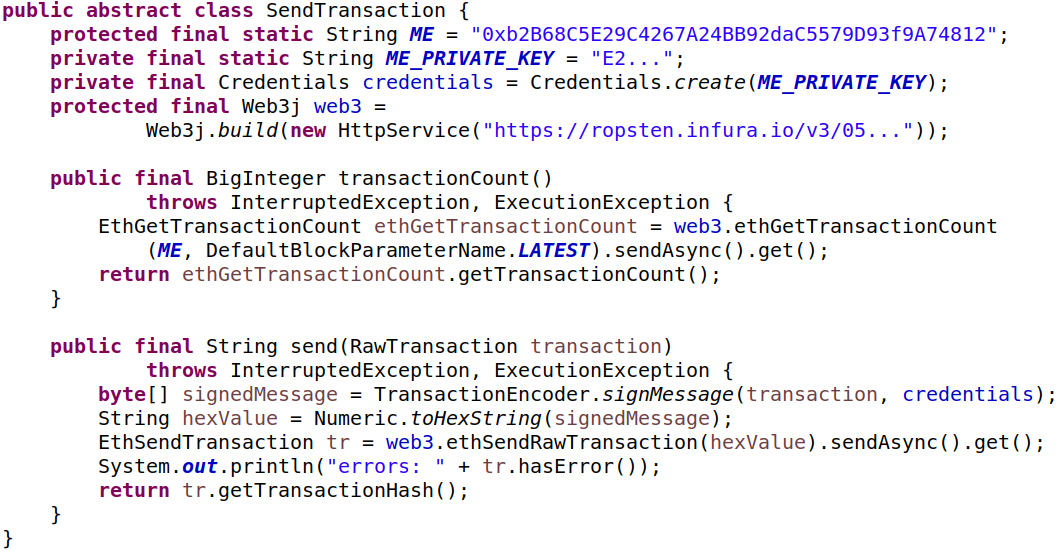
\includegraphics[width=\textwidth,clip=false]{pictures/send-transaction-java.png}
  \end{center}

\end{frame}

\begin{frame}\frametitle{Sending ETH from our account to the faucet}

  \begin{center}
    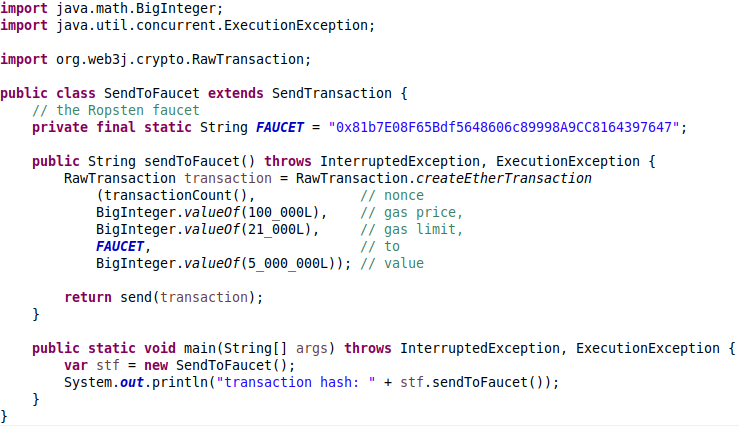
\includegraphics[width=\textwidth,clip=false]{pictures/send-ether-transaction-java.png}
  \end{center}

\end{frame}

\begin{frame}\frametitle{Transactions with value (\emph{payments})}

  \begin{itemize}
  \item the recipient is an EOA (data will be kept in blockchain, but not used):
    \begin{itemize}
    \item the EOA existed already: its balance gets increased by value
    \item the EOA didn't exist before: its balance is set to value
    \end{itemize}
  \item the recipient is a contract:
    \begin{itemize}
    \item there is data:
      \begin{itemize}
      \item there is a \alert{payable} method specified by the data: it will be  executed, after increasing the contract's balance by value
      \item there is no such method or it is not payable: the transaction fails
      \end{itemize}
    \item there is no data:
      \begin{itemize}
      \item there is a \alert{payable \emph{fallback} function}: it will be executed after
        increasing the contract's balance by value
      \item there is no fallback function: the balance of the contract gets increased by value
      \item there is a fallback function, but it is not payable: the transaction fails
      \end{itemize}
    \end{itemize}
  \end{itemize}

\end{frame}

\begin{frame}\frametitle{Transactions targetting contract methods}

  \begin{itemize}
  \item the signing key specifies the caller
  \item the recipient is the address of the receiving contract of the call
  \item the data component encodes signature and actual arguments of the call
  \end{itemize}

  \bigskip

  \begin{greenbox}{How data is computed}
  \begin{enumerate}
  \item take the callee's signature as a string: \<withdraw(uint256)>
  \item compute its Keccak256 hash
  \item take the first 4 bytes: this is the \emph{function selector}
  \item append the actual arguments, serialized
  \end{enumerate}
  \end{greenbox}

\end{frame}

\begin{frame}\frametitle{Calling \<withdraw()> on a contract installed with Remix}

  \begin{center}
    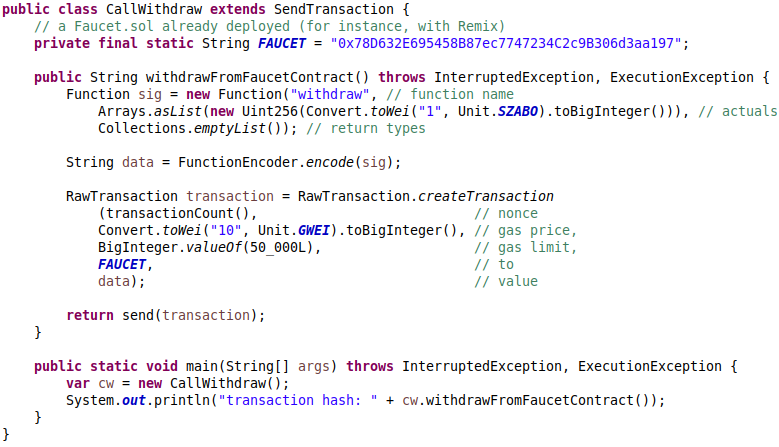
\includegraphics[width=\textwidth,clip=false]{pictures/send-function-transaction-java.png}
  \end{center}

\end{frame}

\begin{frame}\frametitle{Transactions creating a new instance of a contract}

  \begin{itemize}
  \item the signing key specifies the caller
  \item the recipient is set to the zero address
  \item the data component contains the compiled bytecode of the contract
    (ask Remix for that)
  \item the transaction receipt contains the address of the new contract
  \end{itemize}

\end{frame}

\begin{frame}\frametitle{Creating an instance of \<Faucet.sol>}

  \begin{center}
    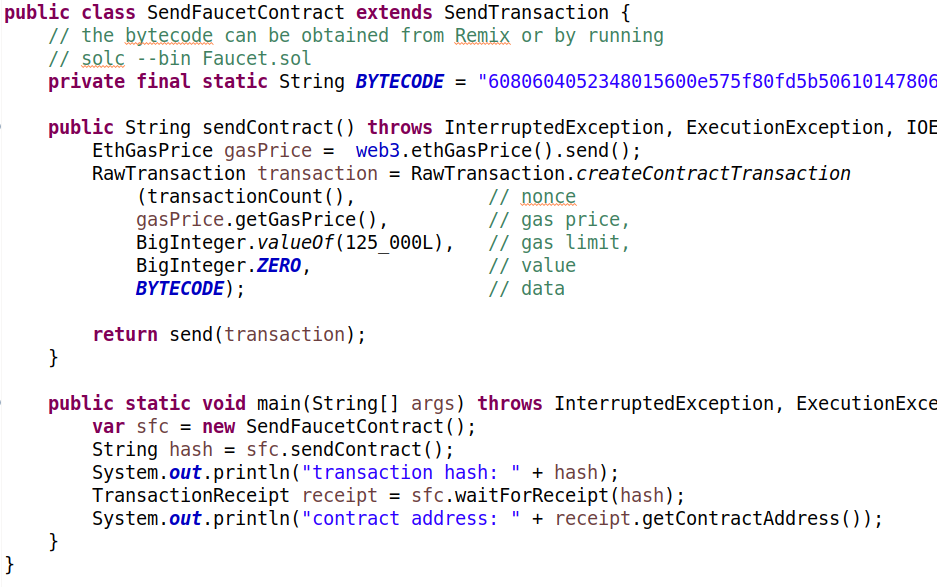
\includegraphics[width=\textwidth,clip=false]{pictures/send-contract-transaction-java.png}
  \end{center}

\end{frame}

\begin{frame}\frametitle{Waiting for the receipt}

  \begin{center}
    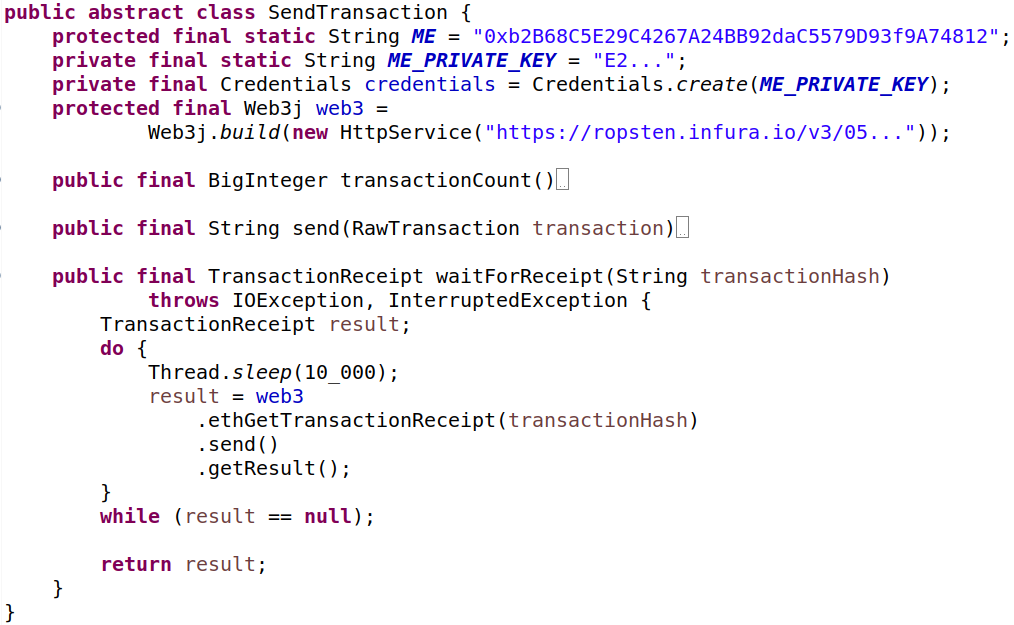
\includegraphics[width=\textwidth,clip=false]{pictures/wait-receipt-java.png}
  \end{center}

\end{frame}

\begin{frame}[fragile]\frametitle{Transaction signing (ECDSA)}

  Transactions are digitally signed before being broadcast to Ethereum:

{\small\begin{verbatim}
Credentials credentials = Credentials.create(ME_PRIVATE_KEY);
byte[] signedMessage = TransactionEncoder.signMessage
  (transaction, credentials);
\end{verbatim}}

  The signature serves three goals:
  \begin{enumerate}
  \item it guarantees that the transaction was created by the sender (\alert{authenticity})
  \item it guarantees that the sender cannot deny having sent the transaction (\alert{non-repudiation})
  \item it guarantees that the transaction was not altered in transit (\alert{integrity})
  \end{enumerate}

  \bigskip

  \begin{greenbox}{}
    The public key of the signer can be recovered from the signed transaction.
    A numerical \alert{chain identifier} is added to the transaction before signing,
    so that transactions cannot be replayed across networks
    (mainnet, testnets\ldots)
  \end{greenbox}
\end{frame}

\begin{frame}\frametitle{Multi-signature transactions}

  \begin{greenbox}{}
    Differently from Bitcoin, Ethereum has no native support for multi-signature transactions
    (that is, transactions that are only valid if signed by more EOAs). However,
    multi-signature and other signature schemes can be programmed through smart contracts:

    \begin{itemize}
    \item extreme flexibility
    \item risk of bugs
    \end{itemize}
      
  \end{greenbox}

  \bigskip

  \begin{center}
    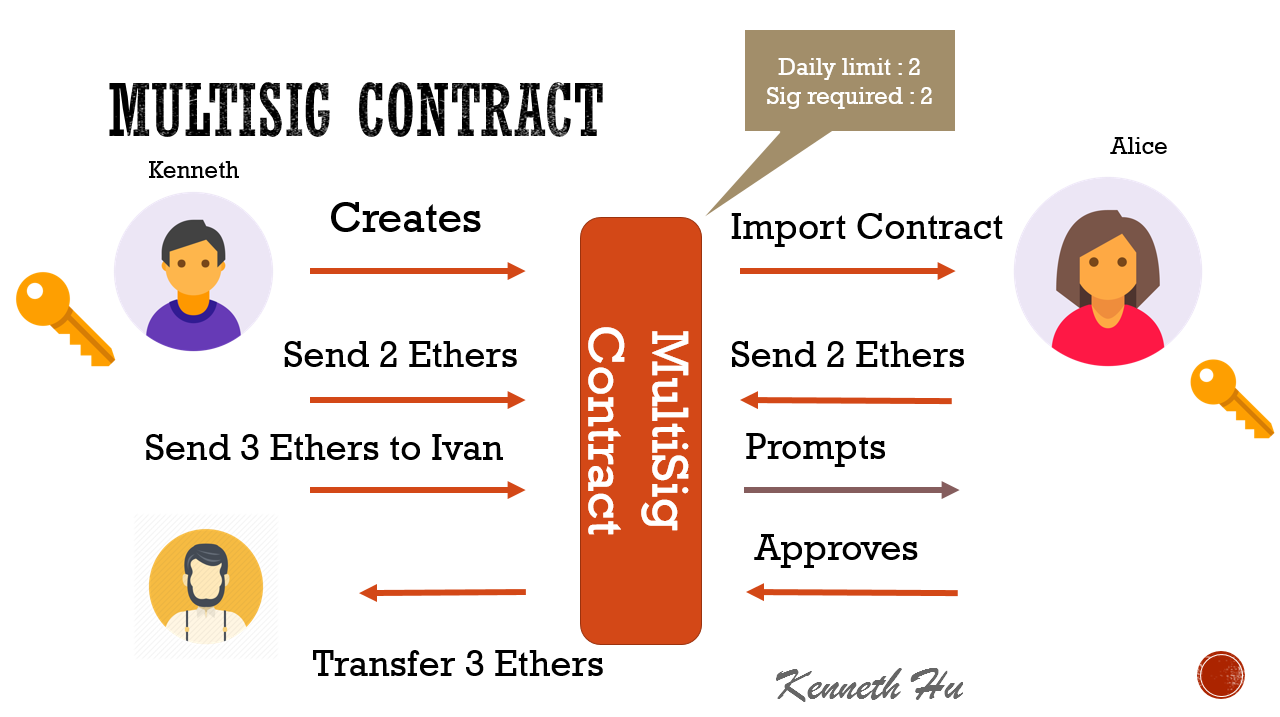
\includegraphics[scale=0.15,clip=false]{pictures/multi-signature.png}
  \end{center}

\end{frame}

\begin{frame}\frametitle{The state of Ethereum}

  \begin{center}
    The state of Ethereum is a global singleton map {\color{magenta}$\sigma:\mathit{key}\to\mathit{value}$}
  \end{center}

  \bigskip

  \begin{redbox}{The state is not in blockchain!}
    Each node keeps and maintains its own copy in a private database
  \end{redbox}

  \bigskip

  \begin{greenbox}{API of the state}
    \begin{enumerate}
    \item \<value=get(address)>
    \item \<put(address, value)>
    \end{enumerate}
  \end{greenbox}

\end{frame}

\begin{frame}\frametitle{Encoding data into the state}

  \begin{greenbox}{Store the balance of an EOA}
    \begin{center}
      \<put(address\_of\_EOA, balance)>
    \end{center}
  \end{greenbox}

  \bigskip

  \begin{greenbox}{Read the balance of an EOA}
    \begin{center}
      \<get(address\_of\_EOA)>
    \end{center}
  \end{greenbox}

\end{frame}

\begin{frame}\frametitle{Encoding data into the state}

  \begin{greenbox}{EOA installs a smart contract}
    \begin{center}
      \<put(>{\color{blue}$\underbrace{\<hash(address\_of\_EOA, nonce\_of\_EOA)>}_{\mathit{address\ of\ the\ new\ smart\ contract}}$}\<, bytecode\_of\_smart\_contract)>
    \end{center}
  \end{greenbox}

  \bigskip

  \begin{greenbox}{A smart contract writes $v$ into its $n$th instance variable (field)}
    \begin{center}
      \<put(>{\color{blue}$\underbrace{\<hash(address\_of\_smart\_contract, n)>}_{\mathit{address\ of\ the\ n-th\ field}}$}\<, v)>
    \end{center}
  \end{greenbox}

  \bigskip

  \begin{greenbox}{A smart contract reads from its $n$th instance variable (field)}
    \begin{center}
      \<get(>{\color{blue}$\underbrace{\<hash(address\_of\_smart\_contract, n)>}_{\mathit{address\ of\ the\ n-th\ field}}$}\<)>
    \end{center}
  \end{greenbox}

\end{frame}

\begin{frame}\frametitle{The hash of the state}

  \begin{greenbox}{In \alert{Bitcoin}, the header of a block contains the hash \alert{of the transactions} in the block}
    That is, the head of the Merkle tree of transactions. Miners must execute
    the transactions to validate them, since invalid transactions would make the whole block invalid,
    which would make the miner lose money
  \end{greenbox}

  \bigskip

  \begin{greenbox}{In \alert{Ethereum}, the header of a block contains the hash \alert{of the state} at the end of the execution of the transactions in the block}
    Since syntactically correct transactions are always valid, this obliges the miners to execute the transactions
  \end{greenbox}

  \bigskip

  \begin{greenbox}{API of the state}
    \begin{enumerate}
    \item \<value=get(address)>
    \item \<put(address, value)>
    \item \<h=get\_hash()>
    \end{enumerate}
  \end{greenbox}

\end{frame}

\begin{frame}\frametitle{The state of a node must change across different views}

  \begin{center}
    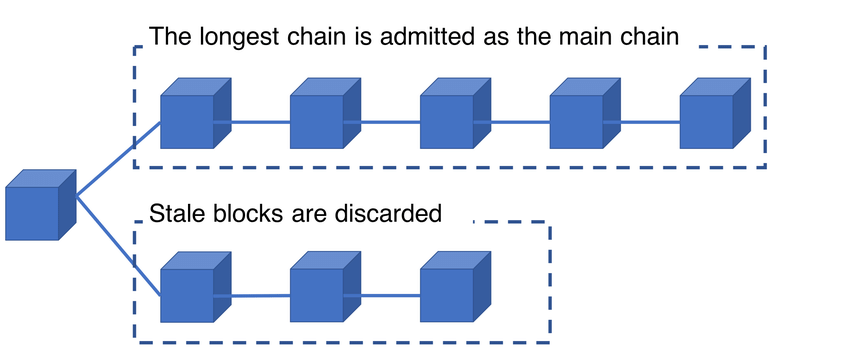
\includegraphics[width=\textwidth,clip=false]{pictures/longest.png}
  \end{center}

  \bigskip

  \begin{itemize}
  \item[] {\color{red}Bitcoin:} (kind of) nothing to do
  \item[] {\color{red}Ethereum:} hard: method executions undo, others must be done
  \end{itemize}

\end{frame}

\begin{frame}\frametitle{Change view to the state at the end of a block}

  \begin{greenbox}{Undo of state updates, up to the state at the end of an old block}
    \begin{center}
      \<checkout(old\_block.header.state\_hash)>
    \end{center}
  \end{greenbox}

  \bigskip

  \begin{greenbox}{The final API of the state}
    \begin{enumerate}
    \item \<value=get(address)>
    \item \<put(address, value)>
    \item \<h=get\_hash()>
    \item \<checkout(h)>
    \end{enumerate}
  \end{greenbox}

\end{frame}

\begin{frame}\frametitle{Ethereum's state is on Git}

  \begin{center}
    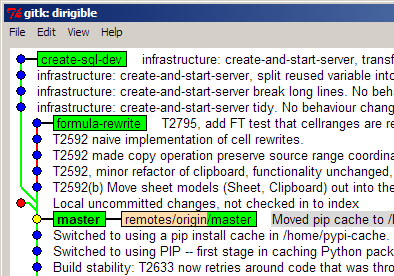
\includegraphics[scale=0.4,clip=false]{pictures/git.png}
  \end{center}

  \bigskip

  \begin{center}
    \<git checkout create-sql-dev>\\
    \medskip
    \<git checkout master>\\
    \medskip
    \<git checkout formula-rewrite>
  \end{center}

\end{frame}

\begin{frame}\frametitle{Merkle-Patricia tries}

  \begin{enumerate}
  \item a compact representation by difference from a previous state
  \item fast recomputation of its hash once the state is updated
  \item fast access to the value bound to each given key
  \item fast change of view
  \end{enumerate}

  \medskip
  Traditional data structures such as hashmaps only satisfy~3
  (and~2, but only for trivial hashing functions, which is not
  acceptable for blockchains)

  \bigskip

  \begin{greenbox}{The final API of the state for keys of length $L$}
    \begin{enumerate}
    \item \<value=get(address)> \hfill $O(L)$
    \item \<put(address, value)> \hfill $O(L+\mathit{size}(\<value>))$
    \item \<h=get\_hash()> \hfill $O(1)$
    \item \<checkout(h)> \hfill $O(1)$
    \end{enumerate}
  \end{greenbox}

\end{frame}

\begin{frame}\frametitle{Patricia trie: fast access to the value bound to each key}

  \begin{center}
    \textbf{P}ractical \textbf{A}lgorithm \textbf{T}o \textbf{R}etrieve \textbf{I}nformation \textbf{C}oded \textbf{I}n \textbf{A}lphanumeric
  \end{center}

  \begin{center}
    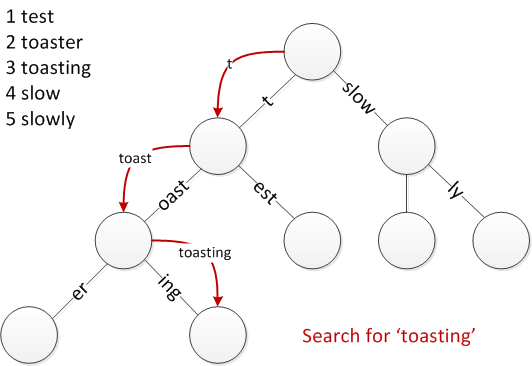
\includegraphics[scale=0.5,clip=false]{pictures/trie_search.png}
  \end{center}

\end{frame}

\begin{frame}\frametitle{Patricia trie: compact representation by difference}

  \begin{center}
    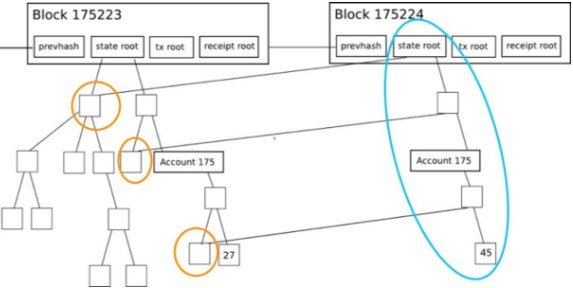
\includegraphics[scale=0.4,clip=false]{pictures/trie-update.jpg}
  \end{center}

\end{frame}

\begin{frame}\frametitle{Merkle trie: fast recomputation of its hash upon update}

  Proceed bottom-up:
  \begin{center}
    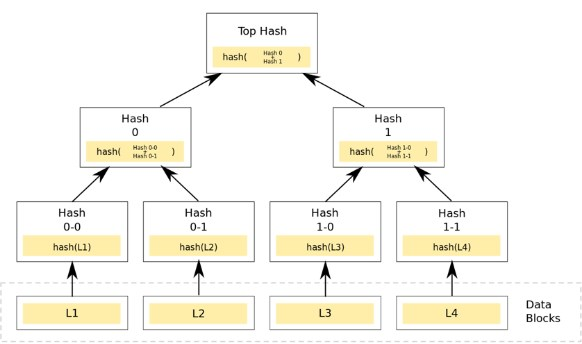
\includegraphics[scale=0.7,clip=false]{pictures/trie-hash.jpg}
  \end{center}

\end{frame}

\begin{frame}\frametitle{Merkle-Patricia tries}

  \begin{center}
    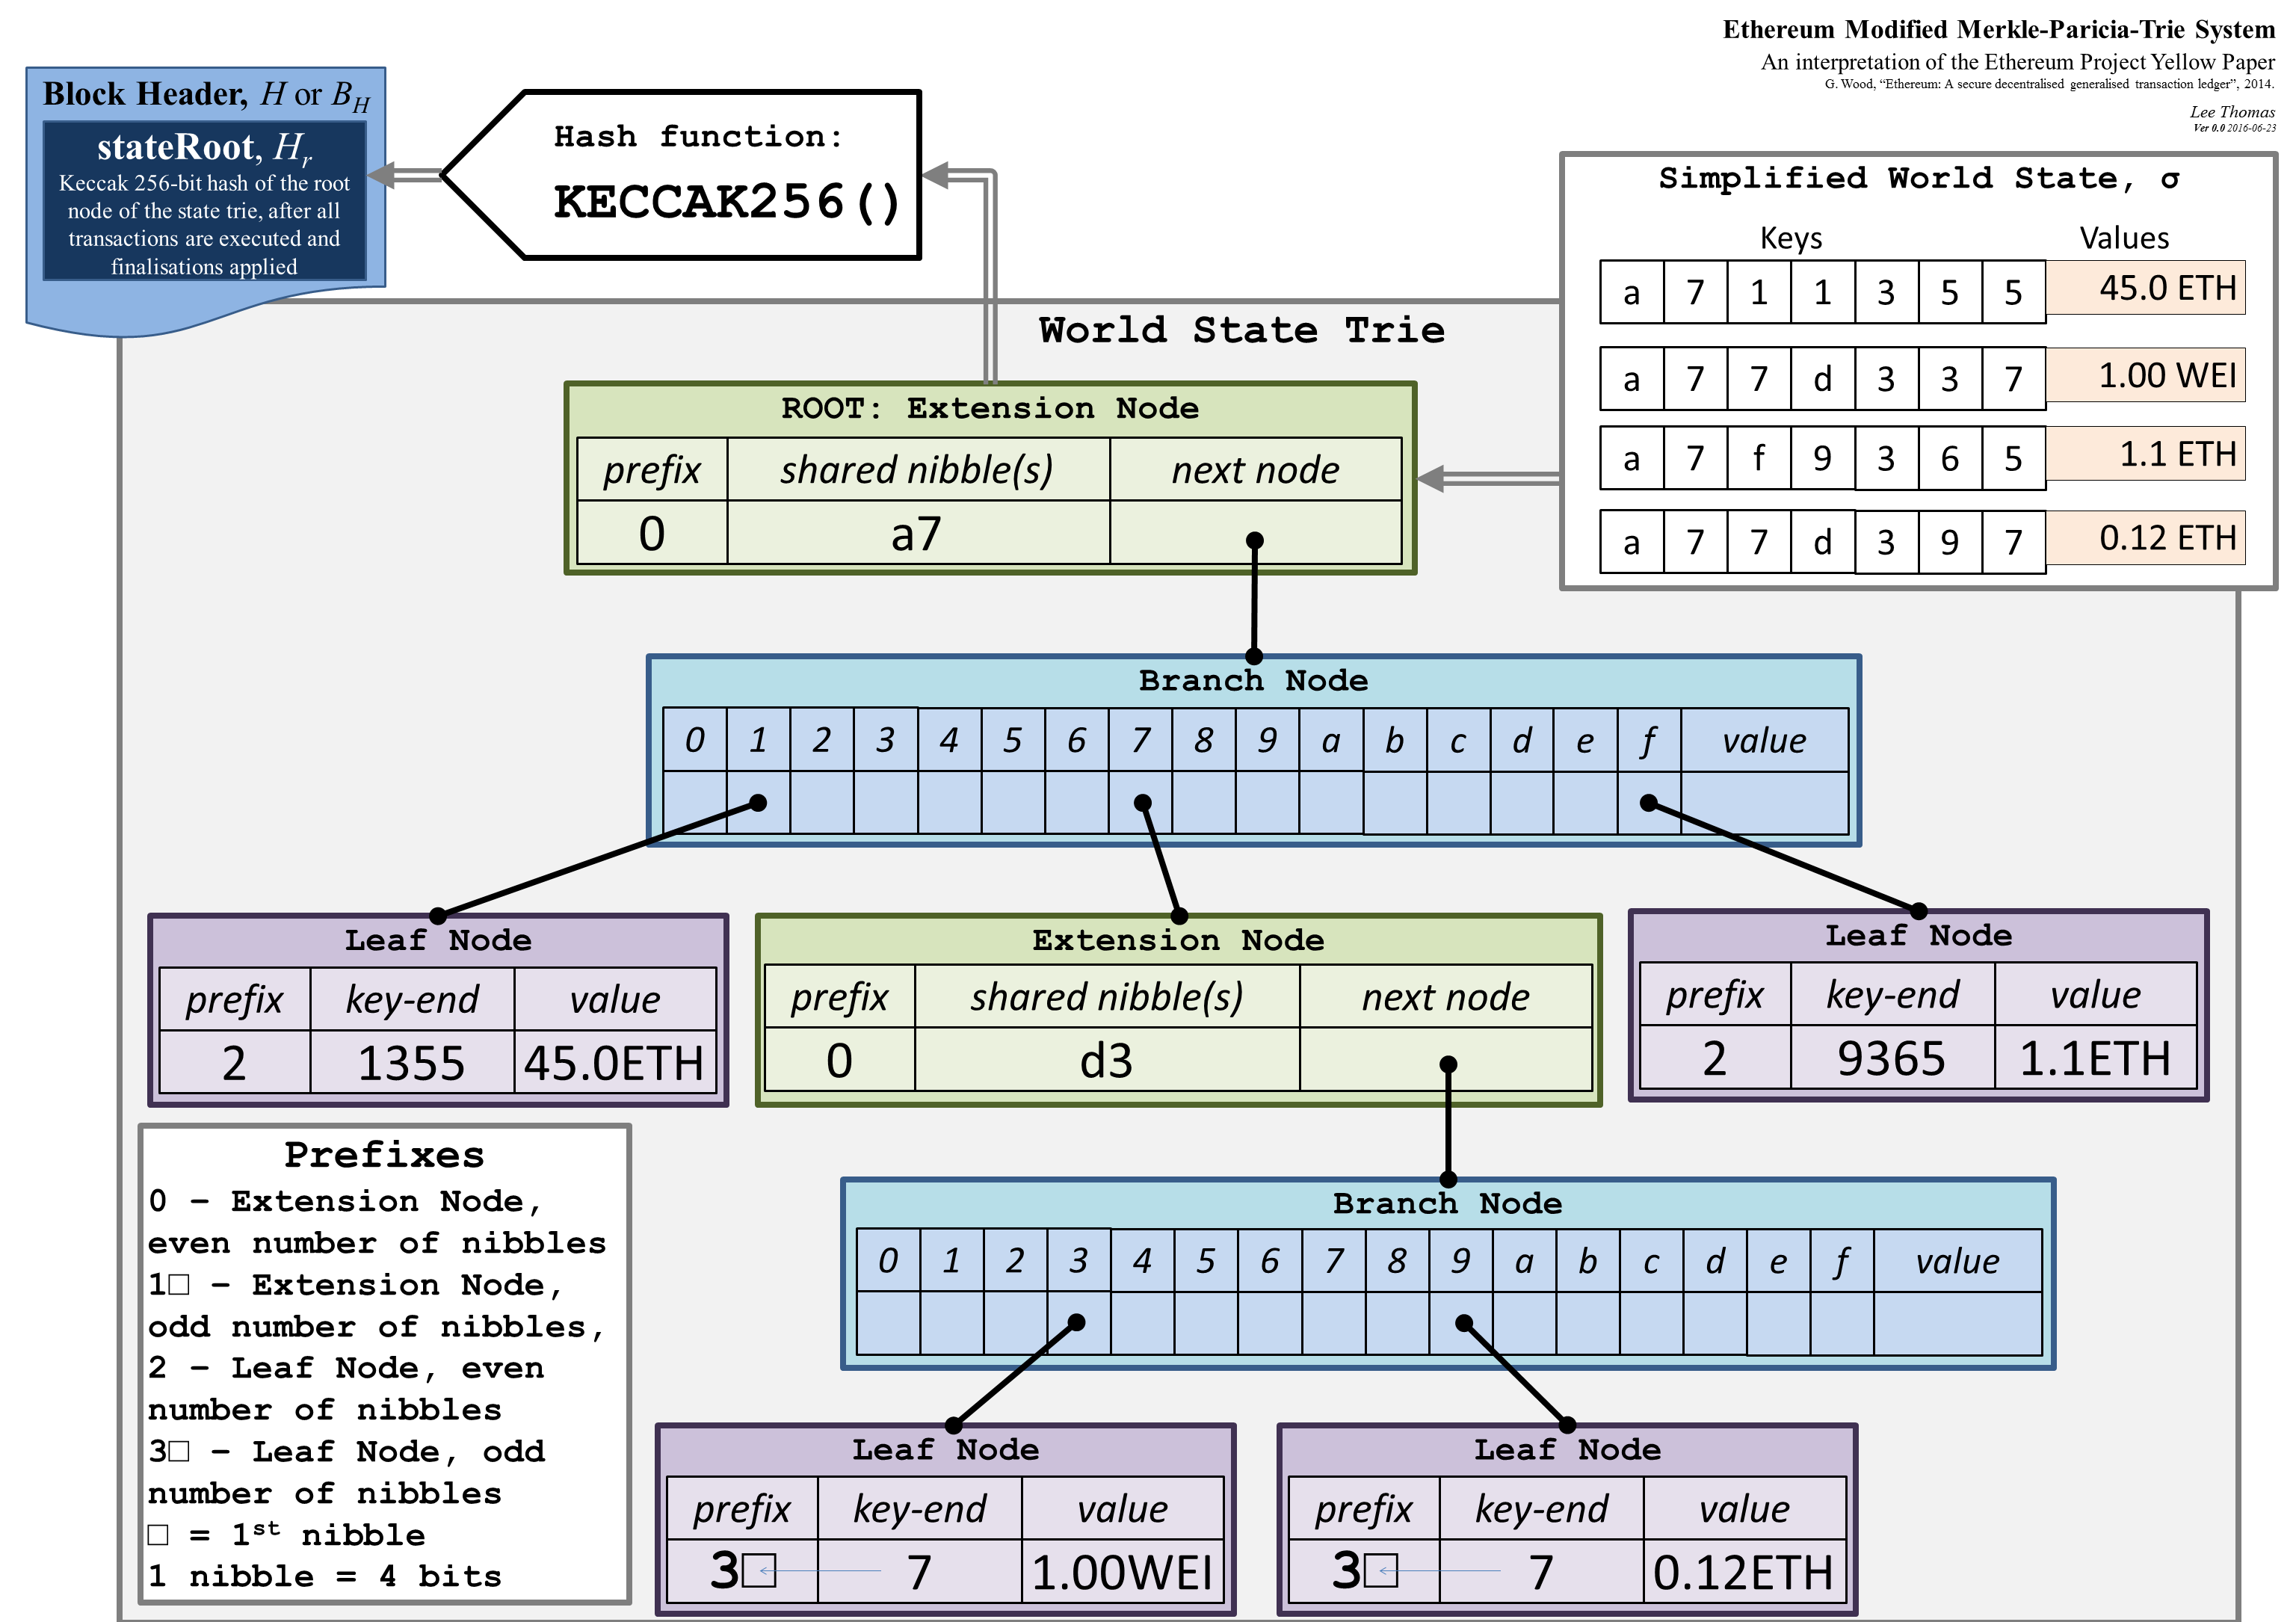
\includegraphics[scale=0.11,clip=false]{pictures/merkle-patricia.png}
  \end{center}

  \begin{center}
    Links are not pointers, but the hash of the node they refer to
  \end{center}

\end{frame}

\begin{frame}\frametitle{A smart contract is\ldots}

  \begin{itemize}
  \item a computer program (not \emph{smart} nor \emph{a contract})
  \item immutable
  \item deterministic
  \item operating on restricted data
  \item running on a decentralized world computer
  \end{itemize}

  In Ethereum:
  \begin{itemize}
  \item compiled into EVM bytecode
  \item installed in blockchain by sending a special transaction to address \<0x0>
  \item its code can be deleted if it executes a \<SELFDESTRUCT> bytecode
  \item has no keys
  \item its installer gets no automatic privileges
  \item runs after a transaction initiated by an EOA
    \begin{itemize}
    \item or a chain of transactions initiated by an EOA
    \item no parallelism, no background processing
    \end{itemize}
  \item transactions are atomic
  \end{itemize}
  
\end{frame}

\begin{frame}\frametitle{Blocks keep transactions not state}

  \begin{center}
    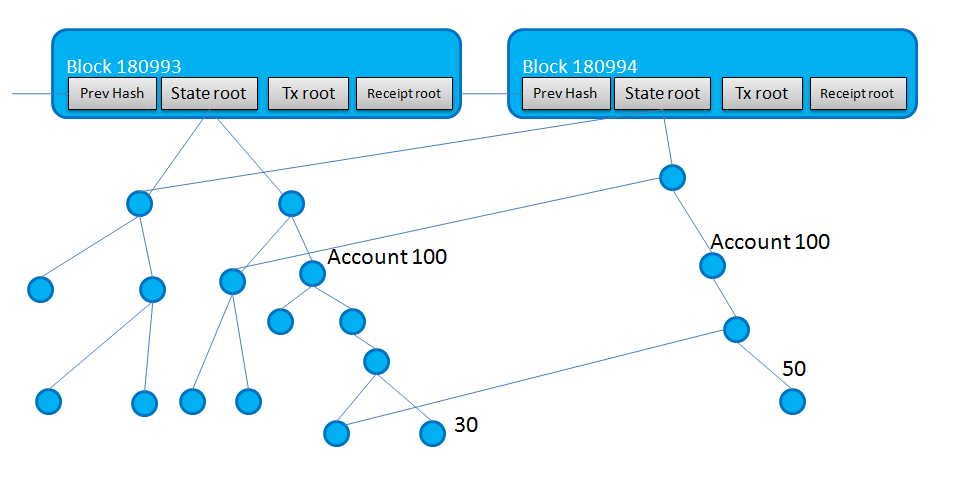
\includegraphics[width=\textwidth,clip=false]{pictures/blocks-state.png}
  \end{center}

  \begin{redbox}{}
    The state root is just a hash of the state tree, to prove that
    transactions have been executed by the miner
  \end{redbox}

\end{frame}

\begin{frame}\frametitle{\<SELFDESTRUCT> has effect on the state}

  \begin{center}
    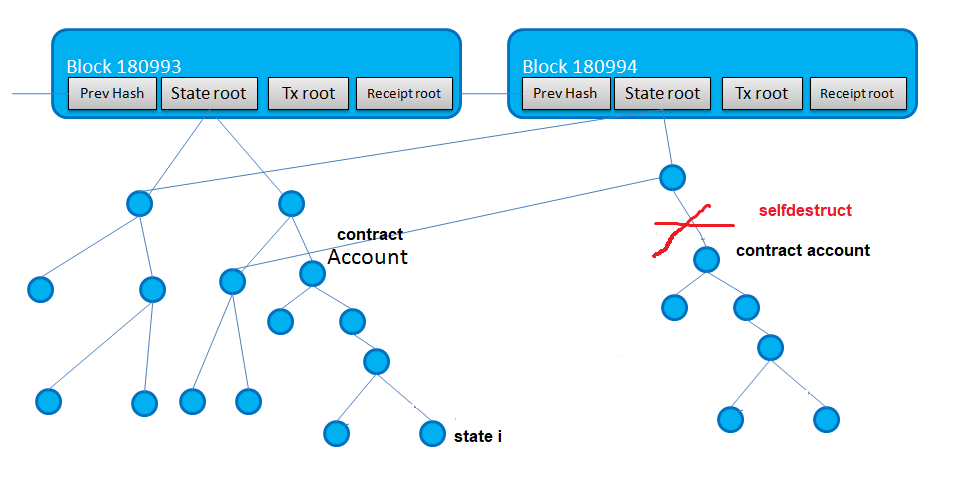
\includegraphics[width=\textwidth,clip=false]{pictures/state-selfdestruct.png}
  \end{center}

\end{frame}

\begin{frame}\frametitle{Solidity}

  \begin{greenbox}{}
    There are many programming languages for Ethereum smart contracts,
    but Solidity is the de facto standard:
    \begin{itemize}
    \item imperative
    \item vaguely object-oriented
    \item in continuous evolution
    \item \alert{non}-strongly-typed
    \item unorthogonal features
    \end{itemize}
  \end{greenbox}

  \bigskip

  \begin{greenbox}{}
    \begin{itemize}
    \item[{\includegraphics[scale=0.03]{pictures/check.png}}] sequence
    \item[{\includegraphics[scale=0.03]{pictures/check.png}}] conditional
    \item[{\includegraphics[scale=0.03]{pictures/check.png}}] repetition
    \end{itemize}

    \begin{center}
      \alert{$\Rightarrow$ Turing complete (bug or feature?)}
    \end{center}

  \end{greenbox}

\end{frame}

\begin{frame}\frametitle{Back to our first Solidity example}
  \begin{center}
    \includegraphics[width=\textwidth,clip=false]{pictures/faucet_sol.png}
  \end{center}
\end{frame}

\begin{frame}[fragile]\frametitle{ABI -- from Remix or from \<solc>}

{\scriptsize\begin{verbatim}
[
  {
    "payable": true,
    "stateMutability": "payable",
    "type": "fallback"
  },
  {
    "constant": false,
    "inputs": [
      {
        "internalType": "uint256",
        "name": "withdraw_amount",
        "type": "uint256"
      }
    ],
    "name": "withdraw",
    "outputs": [],
    "payable": false,
    "stateMutability": "nonpayable",
    "type": "function"
  }
]
\end{verbatim}}
\end{frame}

\begin{frame}[fragile]\frametitle{Select a compiler version}

  \begin{greenbox}{Add a pragma directive}
    \verb!pragma solidity ^0.4.19! requires to compile with a compiler for version $0.4.x$ with $x\ge 19$
  \end{greenbox}

\end{frame}

\begin{frame}\frametitle{Basic Solidity types}
  \begin{greenbox}{\<bool>}
    with constants \<true> and \<false> and usual operators
  \end{greenbox}
  \bigskip
  \begin{greenbox}{\<int>, \<unint>}
    signed or unsigned, with usual operators, in increments of 8 bit size:
    \<uint8>, \<uint16>, \<int24>\ldots. Without specification, they stand for
    \<int256> and \<unint256>, respectively
  \end{greenbox}
  \bigskip
  \begin{greenbox}{\<fixed>$M\times N$, \<ufixed>$M\times N$}
    fixed point arithmetic, signed or unsigned, $M$ bits, $N$ decimals
    after the point: \alert{currently not implemented}
  \end{greenbox}

\end{frame}

\begin{frame}\frametitle{Back to C's \<void *>}

  \begin{greenbox}{\<address>}
    A 20-bytes Ethereum address

    \begin{itemize}
    \item it has a \<balance> field
    \item there is no \<instanceof> operator
    \item casts never fail
    \end{itemize}

  \end{greenbox}

  \bigskip

  \begin{center}
    \includegraphics[scale=0.04,clip=false]{pictures/frog-prince.png}
  \end{center}

  \begin{redbox}{}
    \begin{itemize}
    \item you can dress a frog as a prince, but it will remain a frog
    \item you can dress a prince as a frog, but it will remain a prince
    \item you will understand the difference when you kiss it (segmentation fault)
    \end{itemize}
  \end{redbox}

\end{frame}

\begin{frame}[fragile]\frametitle{Basic Solidity types}

  \begin{greenbox}{\<bytes>$N$}
    fixed-size array of bytes, of length $N$
  \end{greenbox}

  \bigskip

  \begin{greenbox}{\<bytes> or \<string>}
    variable-sized arrays of bytes
  \end{greenbox}

  \bigskip

  \begin{greenbox}{Arrays}
    \<uint32[][5]> is a fixed size array of five dynamic
    arrays of $32$ bits unsigned integers
  \end{greenbox}

  \bigskip

  \begin{greenbox}{Enumerations}
\begin{verbatim}
enum NAME { A, B, ... }
\end{verbatim}
  \end{greenbox}

\end{frame}

\begin{frame}[fragile]\frametitle{Basic Solidity types}

  \begin{greenbox}{Structures}
\begin{verbatim}
struct pair {
  int16 x;
  unint8 y;
}
\end{verbatim}
  \end{greenbox}

  \medskip

  \begin{greenbox}{Mappings}
\begin{verbatim}
mapping(address => unint256) balances;
\end{verbatim}

A field of type mapping spreads its values into the state through hashing:
\<balances[k]=v> executes
\<put(>{{\color{blue}$\underbrace{\<hash(balances,k)>}_{\mathit{address\ of\ \<balances[k]>}}$}}\<, v)>

\begin{itemize}
\item[$\Rightarrow$] mappings default to $0$
\item[$\Rightarrow$] there is no \<containsKey> (you need a sentinel value)
\item[$\Rightarrow$] it is not possible to compute the key set or value set of a mapping
\item[$\Rightarrow$] it is not possible to iterate on a mapping
\end{itemize}
  \end{greenbox}

\end{frame}

\begin{frame}[fragile]\frametitle{Unit multipliers}

  \begin{greenbox}{Time units: \<seconds>, \<minutes>, \<hours>, \<days>}
\begin{verbatim}
uint delay = 3 hours;
\end{verbatim}
  \end{greenbox}

  \bigskip

  \begin{greenbox}{Ether units: \<wei>, \<finney>, \<szabo>, \<ether>}
\begin{verbatim}
require(withdraw_amount <= 0.1 ether);
\end{verbatim}
  \end{greenbox}

\end{frame}

\begin{frame}\frametitle{Transaction information}

  \begin{greenbox}{Structures \<msg> and \<tx> are derived from the transaction request}
    \begin{description}
    \item[\<msg.sender>] the address of the \alert{caller EOA or contract}
    \item[\<msg.value>] the ether sent along the transaction
    \item[\<msg.gasleft>] what remains to consume of the gas limit
    \item[\<msg.data>] the data payload of the transaction
    \item[\<msg.sig>] the first four bytes of \<msg.data> (method selector)
    \item[\<tx.gasprice>] the gas price used for the transaction
    \item[\<tx.origin>] the address of the \alert{originating EOA}
    \end{description}
  \end{greenbox}

\end{frame}

\begin{frame}\frametitle{\<msg.sender> vs \<tx.origin>}

  \begin{center}
    \includegraphics[scale=0.4,clip=false]{pictures/sender-origin.png}
  \end{center}

\end{frame}

\begin{frame}\frametitle{Members of an address}

  \begin{greenbox}{}
    \begin{description}
    \item[\<address.balance>] the balance of the address (EOA or contract),
      such as \<address(this).balance>
    \item[\<address.transfer(x)>] sends $x$ wei to the address; \alert{throws an exception in case of failure}
    \item[\<address.send(x)>] as \<transfer>, but \alert{returns \<false> in case of failure}
    \item[\<address.call(p)>] sends a method transaction to the address, with the given
      payload; \alert{returns \<false> in case of failure}
    \item[\<address.callcode(p)>] sends a method transaction to the address, with the given
      payload; runs in the scope of the caller; \alert{returns \<false> in case of failure}
    \item[\<address.delegatecode(p)>] sends a method transaction to the address, with the given
      payload, but keeps \<msg.sender> and \<msg.value> unchanged;
      runs in the scope of the caller; \alert{returns \<false> in case of failure}
    \end{description}
  \end{greenbox}
  
\end{frame}

\begin{frame}\frametitle{Block information}

  \begin{greenbox}{The structure \<block> is constructed by the miner}
    \begin{description}
    \item[\<block.coinbase>] the address of the miner itself
    \item[\<block.difficulty>] the proof of work difficulty
    \item[\<block.gaslimit>] the maximum gas that can be spent in the current block
    \item[\<block.number>] the current block height
    \item[\<block.timestamp>] the mining time
    \end{description}
  \end{greenbox}

\end{frame}

\begin{frame}\frametitle{Main types in Solidity}

  \begin{description}
  \item[\<contract>] somehow similar to an object in OO-programming. It has a balance
  \item[\<interface>] functions have no code and must be implemented in subtypes
  \item[\<library>] a contract meant to be deployed once and used by other contracts through \<delegatecall>. It has no state variables and no balance. It does not receive ether. It cannot execute \<selfdestruct>.
    \medskip
    \begin{center}
      \includegraphics[scale=0.45,clip=false]{pictures/library.png}
    \end{center}
  \end{description}
  
\end{frame}

\begin{frame}\frametitle{Visibility modifiers}
  \begin{description}
  \item[\<public>] can be called from everywhere
  \item[\<external>] like \<public> but, if called from the same contract,
    must be prefixed with \<this.>, since it triggers a new transaction. It costs less gas than \<public>
  \item[\<internal>] can only be called from the contract where it is defined
    or from its subtypes
  \item[\<private>] can only be called from the contract where it is defined
  \end{description}

  \bigskip

  \begin{redbox}{Privacy?}
    Data is always publicly readable in blockchain. These modifiers
    only refer to who can call whom and are significant for the compiler only
  \end{redbox}
\end{frame}

\begin{frame}\frametitle{Side-effect modifiers}

  \begin{description}
  \item[\<view> or \sout{\<constant>}] the function cannot modify the state
    \begin{center}
      \includegraphics[scale=0.45,clip=false]{pictures/not-view.png}
    \end{center}
  \item[\<pure>] the function cannot modify nor read the state
    \begin{center}
      \includegraphics[scale=0.45,clip=false]{pictures/not-pure.png}
    \end{center}
  \item[\<payable>] the function can receive incoming payments
  \end{description}

\end{frame}

\begin{frame}\frametitle{Specifying return type(s) and value(s)}

  \begin{center}
    \includegraphics[scale=0.52,clip=false]{pictures/returns.png}
  \end{center}

  \bigskip

  \begin{redbox}{\<return> is not mandatory on every execution path}
    When missing, the return value(s) defaults to $0$
  \end{redbox}
\end{frame}

\begin{frame}\frametitle{Constructors}
  \begin{greenbox}{}
    A contract \alert{can} have \alert{up to one} contructor, that gets called
    only once as part of each transaction that deploys an instance
    of the contract
  \end{greenbox}

  \begin{center}
    \includegraphics[scale=0.55,clip=false]{pictures/constructor.png}
  \end{center}

\end{frame}

\begin{frame}\frametitle{Self destruction example}

  Only needed to free state data in clients!

  \begin{center}
    \includegraphics[scale=0.5,clip=false]{pictures/selfdestruct.png}
  \end{center}

\end{frame}

\begin{frame}\frametitle{Self destruction example from 0.6.0}

  \begin{center}
    \includegraphics[scale=0.5,clip=false]{pictures/selfdestruct_6_0.png}
  \end{center}

\end{frame}

\begin{frame}\frametitle{\<address payable>}

  \begin{greenbox}{Starting from 0.5.0, an \<address> can be \<payable>}
    \begin{itemize}
    \item required for calling \<send()>, \<transfer()> and \<call()>
    \item all of \<msg.sender>, \<tx.origin> and \<block.coinbase> are
      \<payable>
    \item you can cast between \<address> and \<address payable> and casts never fail
    \end{itemize}
  \end{greenbox}

  \bigskip

  \begin{greenbox}{Starting from 0.6.0, a contract can have at most
      a \<receive> function}
    \begin{itemize}
    \item it must be \<external payable>
    \item called for transactions without data
    \end{itemize}
  \end{greenbox}

  \bigskip

  \begin{greenbox}{Starting from 0.6.0, a contract can have at most
      a \<fallback> function}
    \begin{itemize}
    \item it must be \<external>
    \item called for transactions with data targetting no function in the
      contract or for transactions without data if there is no \<receive>
      function
    \end{itemize}
  \end{greenbox}

\end{frame}

\begin{frame}\frametitle{Modifiers}

  \begin{greenbox}{They can be used to weave aspects into code}
    \begin{center}
      \includegraphics[scale=0.4,clip=false]{pictures/modifier.png}
    \end{center}
  \end{greenbox}

\end{frame}

\begin{frame}\frametitle{Modifiers}

  \begin{greenbox}{They can be used to do rather weird things}
    \begin{center}
      \includegraphics[scale=0.6,clip=false]{pictures/twice.png}
    \end{center}
  \end{greenbox}

\end{frame}

\begin{frame}\frametitle{Contract extension and inheritance (also multiple)}

  \begin{greenbox}{}
    \begin{center}
      \includegraphics[scale=0.38,clip=false]{pictures/subcontracts.png}
    \end{center}
  \end{greenbox}

\end{frame}

\begin{frame}\frametitle{Constructor chaining}

  \begin{greenbox}{}
    \begin{center}
      \includegraphics[scale=0.5,clip=false]{pictures/constructor_chaining.png}
    \end{center}
  \end{greenbox}

\end{frame}

\begin{frame}\frametitle{Assertions}
  \begin{greenbox}{\<require(condition[,msg])>}
    Evaluates the condition, \alert{that could reasonably not hold}.
    If false, an exception is thrown and the
    transaction is reverted. Typically used for checking user input
  \end{greenbox}

  \bigskip

  \begin{greenbox}{\<assert(condition[,msg])>}
    Evaluates the condition, \alert{that is expected to hold}.
    If false, an exception is thrown and the
    transaction is reverted. Typically used to verify internal runtime conditions
    for debugging
  \end{greenbox}

  \bigskip

  \begin{greenbox}{\<revert([msg])> or {\sout{\<throw>}}}
    Throws an exception and reverts the current transaction
  \end{greenbox}

  \bigskip

  \begin{redbox}{}
    \begin{center}
      There is no way to catch exceptions
    \end{center}
  \end{redbox}

\end{frame}

\begin{frame}\frametitle{Events}

  \begin{greenbox}{}
    \begin{center}
      \includegraphics[scale=0.5,clip=false]{pictures/events.png}
    \end{center}
  \end{greenbox}

  \bigskip

  \begin{center}
    DApps can listen and react to events
  \end{center}

\end{frame}

\begin{frame}\frametitle{Specifying gas and value for inner transactions}

  \begin{greenbox}{\<o.foo(pars)> can be decorated}
    \begin{itemize}
    \item \<o.foo.value(v)(pars)>
    \item \<o.foo.gas(g)(pars)>
    \item \<o.foo.gas(g).value(v)(pars)>
    \end{itemize}
  \end{greenbox}

  \bigskip

  \begin{greenbox}{\<new C(pars)> can be decorated}
    \begin{itemize}
    \item \<(new C).value(v)(pars)>
    \item \<(new C).gas(g)(pars)>
    \item \<(new C).gas(g).value(v)(pars)>
    \end{itemize}
  \end{greenbox}

\end{frame}

\begin{frame}\frametitle{Contract creation and function calls}

  \begin{greenbox}{}
    \begin{center}
      \includegraphics[scale=0.55,clip=false]{pictures/new-contract.png}
    \end{center}
  \end{greenbox}

  \bigskip

  \begin{center}
    In this case, we know what gets called with \<faucet.destroy()>
  \end{center}

\end{frame}

\begin{frame}\frametitle{Contract creation with payable constructor}

  \begin{greenbox}{If the constructor of \<Faucet> were made \<payable>}
    \begin{center}
      \includegraphics[scale=0.5,clip=false]{pictures/new-contract-payable.png}
    \end{center}
  \end{greenbox}

  \bigskip

  \begin{center}
    Also in this case, we know what gets called with \<faucet.destroy()>
  \end{center}

\end{frame}

\begin{frame}\frametitle{Casts do not fail in Solidity}

  \begin{center}
    \includegraphics[scale=0.45,clip=false]{pictures/cast-does-not-fail.png}
  \end{center}

  Calling \<d.callFoo(c)>, where \<c> is a \<C>,
  does not fail but calls \<C>'s
  fallback function and transfers $100$ wei to \<c>!
\end{frame}

\begin{frame}\frametitle{Parameter contract types are just casts}

  \begin{center}
    \includegraphics[scale=0.45,clip=false]{pictures/cast-does-not-fail2.png}
  \end{center}

  Calling \<d.callFoo(c)>, where \<c> is a \<C>,
  does not fail but calls \<C>'s
  fallback function and transfers $100$ wei to \<c>!
\end{frame}

\begin{frame}\frametitle{Solidity is \alert{not} strongly-typed}

  \begin{enumerate}
  \item casts are not checked
  \item parameter types are just Christmas decorations
  \end{enumerate}

  \bigskip

  \begin{redbox}{}
    Remember that a function declaring a formal parameter of type
    \<address> or explicitly \<C> can actually receive any contract, of any
    type, also completely unrelated to \<C>.
    Callers can inject malicious code through such parameters!
  \end{redbox}

  \begin{center}
    \includegraphics[scale=0.28,clip=false]{pictures/frightened-cat.jpg}
  \end{center}

\end{frame}

\begin{frame}\frametitle{Members of an address for low-level calls}

  \begin{greenbox}{}
    \begin{description}
    \item[\<address.call(p)>] sends a method transaction to the address, with the given
      payload; returns \<false> in case of failure. This is actually used
      by the compiler when we write normal function calls
    \item[\<address.callcode(p)>] sends a method transaction to the address, with the given
      payload; runs in the scope of the caller; returns \<false> in case of failure
    \item[\<address.delegatecode(p)>] sends a method transaction to the address, with the given
      payload, but keeps \<msg.sender> and \<msg.value> unchanged;
      runs in the scope of the caller; returns \<false> in case of failure
    \end{description}
  \end{greenbox}
  
\end{frame}

\begin{frame}\frametitle{Example of function call}
  \begin{center}
    \includegraphics[scale=0.35,clip=false]{pictures/normal-call.png}
  \end{center}

  Calling \<d.callSetN(e, 42)> where \<e> is a \<E>:
  \begin{itemize}
  \item \<e.n> will become $42$
  \item \<e.sender> will become \<d>
  \item \<d.n> and \<d.sender> are not modified
  \end{itemize}
\end{frame}

\begin{frame}\frametitle{The previous example is actually compiled into this}

  \begin{center}
    \includegraphics[scale=0.35,clip=false]{pictures/call.png}
  \end{center}

  Calling \<d.callSetN(e, 42)> where \<e> is a \<E>:
  \begin{itemize}
  \item \<e.n> will become $42$
  \item \<e.sender> will become \<d>
  \item \<d.n> and \<d.sender> are not modified
  \end{itemize}
  
\end{frame}

%\begin{frame}\frametitle{Example of a failing low-level \<call>}

%  \begin{center}
%    \includegraphics[scale=0.35,clip=false]{pictures/call.png}
%  \end{center}

%  Calling \<d.callSetN(c, 42)> where \<c> has no \<setN(uint \_n)> function:
%  \begin{itemize}
%  \item the outer transaction will succeed
%  \item the inner \<\_e.call> transaction will fail and be reverted
%  \item function \<\_e.call> will return \<false>
%  \end{itemize}
  
%\end{frame}

\begin{frame}\frametitle{Example of low-level \<callcode>}

  \begin{center}
    \includegraphics[scale=0.35,clip=false]{pictures/callcode.png}
  \end{center}

  Calling \<d.callSetN(e, 42)> where \<e> is a \<E>:
  \begin{itemize}
  \item \<d.n> will become $42$
  \item \<d.sender> will become \<d>
  \item \<e.n> and \<e.sender> are not modified
  \end{itemize}
  
\end{frame}

\begin{frame}\frametitle{Example of low-level \<delegatecall>}

  \begin{center}
    \includegraphics[scale=0.3,clip=false]{pictures/delegatecall.png}
  \end{center}

  Calling \<c.foo(d, e, 42)> where \<d> is a \<D> and \<e> is a \<E>:
  \begin{itemize}
  \item \<d.n> will become $42$
  \item \<d.sender> \alert{will become \<c>}
  \item \<e.n> and \<e.sender> are not modified
  \end{itemize}
  
\end{frame}

\begin{frame}\frametitle{Gas consumption}

  \begin{greenbox}{Each bytecode instruction and transaction type has a gas cost}
    \begin{itemize}
    \item it is possible to compute in advance the gas cost \alert{of simple functions}
      (use \<estimateGas> of web3 for instance)
    \item \alert{the result is wrong in the presence of loops or recursion!}
      \begin{itemize}
      \item obvious, since gas cost computation is equivalent to complexity analysis
        which can be used to decide termination of programs
        \begin{itemize}
        \item[$\Rightarrow$] an algorithm for computing gas costs in advance cannot exist
        \end{itemize}
      \end{itemize}
    \item in general, it is important to know which operations (might) cost much gas, and avoid them
      \begin{itemize}
      \item loops over unbounded dynamic arrays
      \item calls to unknown contracts
      \end{itemize}
    \end{itemize}
  \end{greenbox}
\end{frame}

\begin{frame}\frametitle{A simple Ponzi scheme}

  \begin{center}
    \includegraphics[width=\textwidth,clip=false]{pictures/simple-ponzi.png}
  \end{center}

  \begin{center}
    The first investment will be burned to address \<0x0>
  \end{center}
  
\end{frame}

\begin{frame}\frametitle{Exercise}
  \begin{enumerate}
  \item create an account with MetaMask
  \item charge it from the Ropsten faucet with 1 ETH
  \item write the \<SimplePonzi.sol> contract in Remix
  \item compile the contract in Remix
  \item deploy the contract in Ropsten with Remix
  \item connect to the contract in Ropsten by somebody else
  \item start calling the fallback function with increasing value
    (with Remix of with MetaMask; for the latter, remember to increase
    to gas limit for sending ETH)
  \end{enumerate}

  \bigskip
  You can check the current investment and investor from Remix

\end{frame}

\begin{frame}\frametitle{A gradual Ponzi scheme}

  \begin{center}
    \includegraphics[scale=0.4,clip=false]{pictures/gradual-ponzi.png}
  \end{center}

\end{frame}

\begin{frame}\frametitle{A simple lottery (1)}

  \begin{center}
    \includegraphics[scale=0.4,clip=false]{pictures/simple-lottery-1.png}
  \end{center}

  \begin{center}
    \<now> is the timestamp of the block where the transaction is mined
  \end{center}

\end{frame}

\begin{frame}\frametitle{A simple lottery (2)}

  \begin{center}
    \includegraphics[scale=0.45,clip=false]{pictures/simple-lottery-2.png}
  \end{center}

\end{frame}

\begin{frame}\frametitle{A simple lottery (3)}

  \begin{center}
    \includegraphics[scale=0.45,clip=false]{pictures/simple-lottery-3.png}
  \end{center}

\end{frame}

\begin{frame}\frametitle{A simple lottery (4)}

  \begin{center}
    \includegraphics[scale=0.45,clip=false]{pictures/simple-lottery-4.png}
  \end{center}

\end{frame}

\begin{frame}\frametitle{Exercise}
  \begin{enumerate}
  \item create an account with MetaMask
  \item charge it from the Ropsten faucet with 1 ETH
  \item write the \<SimpleLottery.sol> contract in Remix
  \item compile the contract in Remix
  \item deploy the contract in Ropsten with Remix, with 3 minutes for buying tickets
  \item connect to the contract in Ropsten by somebody else
  \item buy some tickets before the 3 minutes expire
    (with Remix or with MetaMask; for the latter, remember to increase
    to gas limit for sending ETH)
  \item the owner of the lottery contract draws the winner
  \item try to withdraw your price (if any!)
  \end{enumerate}

  \medskip
  You can check the winner from Remix

\end{frame}

\begin{frame}\frametitle{A simple auction (1)}

  \begin{center}
    \includegraphics[scale=0.55,clip=false]{pictures/simple-auction-1.png}
  \end{center}

\end{frame}

\begin{frame}\frametitle{A simple auction (2)}

  \begin{center}
    \includegraphics[scale=0.48,clip=false]{pictures/simple-auction-2.png}
  \end{center}

\end{frame}

\begin{frame}\frametitle{A simple auction (3)}

  \begin{center}
    \includegraphics[scale=0.45,clip=false]{pictures/simple-auction-3.png}
  \end{center}

\end{frame}

\begin{frame}\frametitle{A simple auction (4)}

  \begin{center}
    \includegraphics[scale=0.52,clip=false]{pictures/simple-auction-4.png}
  \end{center}

\end{frame}

\begin{frame}\frametitle{Why this complicated withdraw pattern?}

  \begin{center}
    \includegraphics[scale=0.5,clip=false]{pictures/simple-auction-withdraw.png}
  \end{center}

\end{frame}

\begin{frame}\frametitle{Why this complicated withdraw pattern?}

  \begin{greenbox}{\<highestBidder.transfer(highestBid); DON'T DO THIS!!!>}
    The problem with this call (inside function \<bid()>) is that
    a broken or malicious bidder might redefine its own fallback function in
    such a way to consume all gas (for instance):
    \begin{itemize}
    \item all subsequent bidders will get a failure when calling \<bid()>
    \item the broken or malicious contract will never be replaced by another bidder
    \end{itemize}
  \end{greenbox}

\end{frame}

\begin{frame}\frametitle{The reentrancy nightmare}

  \only<1>{
  \begin{center}
    \includegraphics[scale=0.50,clip=false]{pictures/simple-auction-withdraw-only.png}
  \end{center}
  }
  \only<2>{
    \begin{center}
      Beware: code vulnerable to reentrancy:\\
    \includegraphics[scale=0.50,clip=false]{pictures/simple-auction-withdraw-only-wrong.png}
  \end{center}
  }

  \only<1>{
    Why this complication of setting \<pendingReturns[msg.sender]=0>
    so early?
  }
    
  \only<2>{
  \begin{greenbox}{Order does matter}
    \begin{itemize}
    \item a malicious bidder might redefine its own fallback function
      in order to call \<withdraw()> back again, as many times as it likes
    \item it will withdraw its \<amount> as many times as it wants, until
      the auction contract is depleted
    \item basically, it runs away with the highest bid and with the bids of all bidders
      that have not been withdrawn yet
    \end{itemize}
  \end{greenbox}
  }

\end{frame}

\begin{frame}\frametitle{The reentrancy nightmare}

  \begin{center}
    \includegraphics[width=\textwidth,clip=false]{pictures/re-entrancy.png}
  \end{center}

\end{frame}

\begin{frame}\frametitle{The DAO attack (2016)}

  \begin{greenbox}{The most famous reentrancy exploit}
    \begin{itemize}
    \item the DAO was a contract for autonomous decentralized organizations
    \item the attacker used reentrancy to steal $50\text{M}\$$ equivalent of ETH
    \item the Ethereum team decided to make the consensus rules more restrictive in order
      to make such transactions illegal and get some of that money back
    \item some node maintainers didn't accept the change and continued
      operating with the old rules and another chain id, leading to a network hard fork known as
      Ethereum Classic
    \end{itemize}
  \end{greenbox}

  \begin{center}
    \includegraphics[scale=0.5,clip=false]{pictures/ethereum-vs-ethereum-classic.jpg}
  \end{center}

\end{frame}

\begin{frame}[fragile]\frametitle{Are \<send()> and \<transfer()> safe from reentrancy?}

  \begin{greenbox}{Currently yes}
    \begin{itemize}
    \item they only forward $2300$ units of gas, not enough for reentrancy
    \item differently from the low-level \verb!msg.sender.call.value(amount)("")!, that forwards all gas and definitely allows reentrancy
    \item however:
      \begin{itemize}
      \item gas costs might change in the future, allowing reentrancy also
        with $2300$ units of gas
      \item the programmer might decide to forward more gas explicitly in order to deal
        with contracts with complex fallback functions
      \item \<send()> and \<transfer()> risk to be deprecated soon\ldots
      \end{itemize}
    \item in conclusion, it's good practice to
      set \<pendingReturns[msg.sender] = 0>
      before sending the money to
      \<msg.sender>, however that last operation is performed
    \end{itemize}
  \end{greenbox}

\end{frame}

\begin{frame}\frametitle{A blind auction (1)}

  \begin{greenbox}{In our simple auction, everything happens in clear}
    We want a \alert{blind auction} now, where:
    \begin{description}
    \item[start] an EOA starts the auction and becomes its owner
    \item[bidding phase] bidders place zero, one or more bids in \alert{closed envelopes};
      some envelopes might contain bids marked as \alert{fake}, which allows one to bluff
    \item[revealing phase] bidders provide the secret needed to open the envelopes
    \item[end] the best non-fake bid is forwarded to the auction's owner
    \end{description}
  \end{greenbox}

  \begin{center}
    \includegraphics[scale=0.1,clip=false]{pictures/blind.jpg}
  \end{center}

\end{frame}

\begin{frame}\frametitle{A blind auction (2)}

  \begin{center}
    \includegraphics[scale=0.5,clip=false]{pictures/blind-auction-1.png}
  \end{center}

\end{frame}

\begin{frame}\frametitle{A blind auction (3)}

  \begin{center}
    \includegraphics[scale=0.42,clip=false]{pictures/blind-auction-2.png}
  \end{center}

\end{frame}

\begin{frame}\frametitle{A blind auction (4)}

  \begin{center}
    \includegraphics[scale=0.35,clip=false]{pictures/blind-auction-3.png}
  \end{center}

\end{frame}

\begin{frame}\frametitle{A blind auction (5)}

  \begin{center}
    \includegraphics[scale=0.5,clip=false]{pictures/blind-auction-4.png}
  \end{center}

\end{frame}

\begin{frame}\frametitle{Exercise}

  \begin{greenbox}{Write a \<TicTacToe.sol> smart contract}
    \begin{itemize}
    \item the first EOA that calls the payable function \<play(x,y)> becomes player~1:
      she must pay at least $0.01$ ETH
    \item the second EOA that calls the payable function \<play(x,y)> becomes player~2:
      he must be different from player~1;
      he must pay at least what player~1 payed
    \item subsequent calls to \<play> do not require any payed amount
    \item if one player wins, the balance of the game goes
      \begin{itemize}
      \item $90\%$ to the winner
      \item $10\%$ to the creator of the game
      \end{itemize}
    \item if the game is a draw, $10\%$ of the balance of the game goes to the creator of the game
    \item after victory or draw, the game resets and is ready to accept new players
    \end{itemize}
  \end{greenbox}

\end{frame}

\begin{frame}\frametitle{Exercise}

  \begin{greenbox}{Write a user interface that connects to the \<TicTacToe.sol> smart contract}
    \begin{itemize}
    \item as a Java textual desktop application using Infura
    \item as a Java graphical desktop application using Infura
    \item as an Android mobile application using Infura
    \item as a web application (Javascript) using Infura
    \item the same as above, but connecting directly to an Ethereum node\ldots
    \end{itemize}
  \end{greenbox}

\end{frame}

\begin{frame}\frametitle{Security best practice}

  \begin{itemize}
  \item Minimalism: the simpler, the better
  \item Code reuse: DRY, use well-known libraries
  \item Study: be aware of well-known issues and solutions
  \item Readability: simpler audit
  \item Test: try corner cases
  \item Analysis: static or dynamic, still in infancy
  \end{itemize}

  \bigskip

  \begin{redbox}{}
    Considering the importance of security for smart contracts,
    it is questionable to have invented Solidity (hard, new, with complex
    semantics) for writing such delicate pieces of software
  \end{redbox}

  \bigskip

  \begin{center}
    Remember the DAO
  \end{center}
  
\end{frame}

\begin{frame}\frametitle{Issue \#1: Reentrancy}

  \begin{redbox}{}
    Our contract calls an unknown contract. The latter, unexpectedly, calls
    back into our contract again. Particularly dangerous if this cycle
    passes through a call sending ETH, that would be repeated as many
    times as the unknown contract decides
  \end{redbox}

  \bigskip

  \begin{greenbox}{Three ways of sending ETH}
    \begin{description}
    \item[\<c.send(amount)>] forwards $2300$ units of gas,
      \alert{currently not enough for reentrancy}; possibly
      deprecated in the future
    \item[\<c.transfer(amount)>] forwards $2300$ units of gas,
      \alert{currently not enough for reentrancy}; possibly
      deprecated in the future
    \item[\<c.call.value(amount)("")>] forwards all remaining units of gas,
      typically \alert{enough for reentrancy}; programmers like it since
      it allows one to activate the complex fallback function of any
      contract, not just the default fallback function
    \end{description}
  \end{greenbox}
  
\end{frame}

\begin{frame}\frametitle{Reentrancy: prevention}

  \begin{greenbox}{Use the checks/effects/interactions pattern}
    \begin{center}
      \includegraphics[scale=0.4,clip=false]{pictures/simple-auction-withdraw-only.png}
    \end{center}
  \end{greenbox}

  \medskip

  \begin{greenbox}{Use a mutex to ban reentrancy}
    \begin{center}
      \includegraphics[scale=0.35,clip=false]{pictures/mutex.png}
    \end{center}
  \end{greenbox}
  
\end{frame}

\begin{frame}\frametitle{Issue \#2: Arithmetic over/underflows}

  \begin{redbox}{}
    An operation tries to compute a fixed-size value that is outside the
    bounds for its type
  \end{redbox}

  \bigskip

  \begin{greenbox}{What if an account with $0$ balance tries to send $1$ ETH to another account?}
    \begin{center}
      \includegraphics[scale=0.5,clip=false]{pictures/under-overflow.png}
    \end{center}
  \end{greenbox}
  
\end{frame}

\begin{frame}\frametitle{Over/underflows: prevention}

  \begin{greenbox}{Test numerical operations}
    \begin{center}
      \includegraphics[scale=0.45,clip=false]{pictures/under-overflow-fixed-check.png}
    \end{center}
  \end{greenbox}
    
\end{frame}

\begin{frame}\frametitle{Over/underflows: prevention}

  \begin{greenbox}{Replace numerical operations with a library for safe arithmetic}
    \begin{center}
      \includegraphics[scale=0.45,clip=false]{pictures/under-overflow-fixed.png}
    \end{center}
  \end{greenbox}
    
\end{frame}

\begin{frame}\frametitle{Over/underflows: prevention}

  \begin{greenbox}{A library for safe arithmetic}
    \begin{center}
      \includegraphics[scale=0.45,clip=false]{pictures/safe-math.png}
    \end{center}
  \end{greenbox}

  \medskip

  \begin{center}
    \url{https://docs.openzeppelin.com/contracts/3.x/api/math}
  \end{center}
  
\end{frame}

\begin{frame}\frametitle{Issue \#3: Unexpected ether}

  \begin{redbox}{}
    Code correctness depends on invariants about \<this.balance>,
    that actually do not hold
  \end{redbox}

  \bigskip

  \begin{greenbox}{This code assumes \<this.balance \% 0.5 ether == 0>. But this is false
      since it is possible to send $0.1$ ether to this contract\ldots}
    \begin{center}
      \includegraphics[scale=0.5,clip=false]{pictures/unexpected-ether.png}
    \end{center}
  \end{greenbox}

\end{frame}

\begin{frame}\frametitle{Issue \# 3: Unexpected ether}

  \begin{redbox}{}
    It is possible to send ether to a contract, without calling any \<payable> function
    nor its fallback function (if any)!
  \end{redbox}

  \bigskip

  \begin{greenbox}{How?}
    \begin{itemize}
    \item write a suicidal contract that executes \<selfdestruct(beneficiary)>
      and forwards its balance to \<beneficiary>: it does not even call
      the fallback function of \<beneficiary>!
    \item mine a block and put the contract as destination coinbase address
      (expensive, but it depends on the final goal\ldots)
    \item let ether be there from the very beginning, by sending ether
      to the address of the contract before its same creation!
      Remember that the address of a contract is computed deterministically
      from the address of the creator and from its current nonce
    \end{itemize}
  \end{greenbox}
  
\end{frame}

\begin{frame}\frametitle{Unexpected ether: prevention}

  \begin{greenbox}{Do not rely on \<this.balance>}
    Use your own counter instead
  \end{greenbox}

  \bigskip

  \begin{center}
    \includegraphics[scale=0.5,clip=false]{pictures/unexpected-ether-fixed.png}
  \end{center}  

\end{frame}

\begin{frame}\frametitle{Issue \#4: \<delegatecall>}

  It is a low-level call that allows one to call any method, as
  done in Java by reflection (actually much worse than reflection)

  \bigskip

  \begin{redbox}{It keeps the calling context}
    If the callee reads/modifies its $n$th state variable, it actually
    reads/modifies the $n$th state variable of the caller, regardless of
    names and types
  \end{redbox}

\end{frame}

\begin{frame}\frametitle{Example: storage slot clash}

  \begin{center}
    \includegraphics[scale=0.33,clip=false]{pictures/delegatecall-storage-clash.png}
  \end{center}

  By invoking the constructor of \<Caller> with the address of a \<Callee> \only<1>{\ldots}\visible<2>{one actually
  sets the \alert{\<private>} field \<lib> of the \<Caller> to $42$

  \begin{center}
    \includegraphics[scale=0.35,clip=false]{pictures/surprised-cat.jpg}
  \end{center}}

\end{frame}

\begin{frame}\frametitle{Example: call injection}

  \begin{center}
    \includegraphics[scale=0.5,clip=false]{pictures/delegatecall-call-injection.png}
  \end{center}

  The caller can forge proper data so that \<delegatecall> ends up calling
  everything!

  \bigskip

  The same can occur with all low-level calls

\end{frame}

\begin{frame}\frametitle{\<delegatecall>: prevention}

  \begin{greenbox}{}
    \begin{itemize}
    \item use it only on \<library>s: they cannot have state, hence they do not read/modify fields
      \begin{itemize}
      \item double-check that the receiver cannot be injected
      \end{itemize}
    \item use it with prepared call data only, to avoid call injections
    \item let the compiler, not you, use it, to compile calls to \<library>s
    \end{itemize}
  \end{greenbox}

\end{frame}

\begin{frame}\frametitle{Issue \#5: Weak encapsulation}

  \begin{greenbox}{}
    Programmers tend to be too permissive about visibility modifiers, often because
    they get along with the default \<public> visibility
  \end{greenbox}

  \begin{center}
    \includegraphics[scale=0.4,clip=false]{pictures/weak-visibility.png}
  \end{center}

  \begin{redbox}{}
    \begin{center}
      Everybody can call \<sendWinnings()>, it \sout{is} was \<public> by default!
    \end{center}
  \end{redbox}

  \medskip

  \begin{greenbox}{}
    Too stupid? Do not overestimate the intelligence of
    programmers: somebody stole $\$31\text{M}$ from
    a slightly more complex contract than this
  \end{greenbox}

\end{frame}

\begin{frame}\frametitle{Weak encapsulation: prevention}

  \begin{itemize}
  \item be the stricter you can about visibility
    \begin{itemize}
    \item even \<internal> can be dangerous, because it is callable from
      subcontracts
    \end{itemize}
  \item beware of default visibility (\emph{ie.}, \<public>)
    \begin{itemize}
    \item latest compilers forbid default visibility
    \end{itemize}
  \item think seriously about the API of your contracts
  \end{itemize}

  \bigskip

  \begin{redbox}{}
    What, in traditional software development,
    is \emph{just} a question of style, order and good engineering,
    becomes here a question of MONEY
  \end{redbox}

\end{frame}

\begin{frame}\frametitle{Issue \#6: Entropy illusion}

  \begin{redbox}{Nothing is really random in blockchain}
    Do not rely on \<block.number>, \<block.gaslimit>, \<block.timestamp> or \<now>
      as a source of randomness: they are (partially) controlled by the miner
  \end{redbox}

  \begin{center}
    \includegraphics[scale=0.42,clip=false]{pictures/roulette.png}
  \end{center}

  The miner might choose \<now> so that the condition holds (or does not hold)
\end{frame}

\begin{frame}\frametitle{Entropy illusion: prevention}

  \begin{greenbox}{}
    \begin{itemize}
      \item use an external trusted \alert{oracle} as a source of randomness:
        \begin{description}
        \item[Oracle] A computer that regularly sends transactions that
          store data in blockchain. For instance, it sends and stores a random number
        \end{description}
      \item if \<now> or \<block.timestamp> is used to wait for a period of time,
        it might be safer to wait for a specific blockchain height instead, since it cannot
        really be controlled by miners
    \end{itemize}
  \end{greenbox}
    
\end{frame}

\begin{frame}\frametitle{Issue \#7: External contract referencing}

  \begin{redbox}{}
    Casts and contract types are unchecked. Do not let clients
    inject contract types through the public API
  \end{redbox}

  \medskip

  \begin{greenbox}{By injecting a malicious \<\_tail>, function \<length> might run
    arbitrary code}
  \begin{center}
    \includegraphics[scale=0.32,clip=false]{pictures/list.png}
  \end{center}
  \end{greenbox}

  \medskip

  \begin{redbox}{}
    This even compiles if \<length> is defined as \<view>, although it can have
    any possible side-effect
  \end{redbox}

\end{frame}

\begin{frame}\frametitle{External contract referencing: prevention}

  \begin{itemize}
  \item avoid it!
  \item do not call functions on externally referenced contracts
  \item only talk to your friends!
    \begin{itemize}
    \item if \<field = new MyContract()> is the only way to initialize \<field>,
      then you can be sure about the run-time type of \<field>
    \end{itemize}
  \end{itemize}
  
\end{frame}

\begin{frame}\frametitle{Issue \#8: Short address/parameter attack}

  \begin{redbox}{}
    Function parameters are encoded as transaction data. If shorter than
    expected, the encoding is silently padded with $0$'s
  \end{redbox}

  \medskip

  \begin{greenbox}{How to buy a Porsche with $1431$ euros}
    \begin{enumerate}
    \item generate private keys until the derived address \<A> ends in \<0x00>
    \item communicate the first $38$ digits \<A'> of \<A> to an exchange (without the
      two final \<0x00>), asking to buy $1$ ETH (as of today, $1431$ euros)
    \item pay the exchange the $1431$ euros (plus commission)
    \item its wallet will prepare a transaction to some
      \<transfer(address to, uint tokens)>, with data
      \<selector::A'::0x000000....00001::0x00>, where the final \<0x00> is padding
      to match the expected data size for \<transfer>
    \item the EVM will interpret the address as \<A'::0x00>, that is, \<A> (ours!)
    \item the EVM will interpret the \<tokens> parameter as $\<0x0000...000100>$, that is,
      $256$ ETH (as of today, $366336$ euros)
    \item you will earn $336336-1431=364905$ euros (minus commission)
    \end{enumerate}
  \end{greenbox}
  
\end{frame}

\begin{frame}\frametitle{Prevention: Short address/parameter attack}

  \begin{greenbox}{Spoiler: exchanges check consistency of data nowadays}
    \begin{center}
      \includegraphics[scale=0.32,clip=false]{pictures/cat-jail.jpg}
    \end{center}
  \end{greenbox}

  \bigskip

  \begin{center}
    Let your applications check parameters passed into blockchain
  \end{center}

\end{frame}

\begin{frame}\frametitle{Issue \#9: Unchecked return value}

  \begin{redbox}{}
    The return value of some functions (typically, \<send> and
    \<call>) should be checked, since it is a boolean
    that informs about their outcome
  \end{redbox}

  \begin{center}
    \includegraphics[scale=0.3,clip=false]{pictures/lotto.png}
  \end{center}

  \begin{center}
    \<payedOut> is set to true even if \<winner.send(winAmount)> fails
  \end{center}

  \medskip

  \begin{greenbox}{}
    Prevention: check the result of \<send> and \<call>. Use \<transfer> instead of \<send>
  \end{greenbox}
\end{frame}

\begin{frame}\frametitle{Issue \#10: Race conditions/front running}

  \begin{redbox}{}
    Miners process transactions fromthe mempool in the order they like (if ever);
    in general, they tend to proceed in decreasing \<gasPrice> order
  \end{redbox}

  \bigskip

  \begin{greenbox}{Scenario \#1 (transaction ban, unlikely)}
    A miner could be instructed to never include a transaction that is
    detrimental to its owner. Unlikely to work for long, since it is practically impossible
    to be the fastest to mine the next block, always
  \end{greenbox}

  \bigskip

  \begin{greenbox}{Scenario \#2 (transaction front running, likely)}
    A network sniffer could scan transactions, looking for
    those containing solutions to priced puzzles, and immediately
    place its own transaction with the same solution but a much higher \<gasPrice>,
    so that all miners will prefer to mine its transaction rather than the
    original one. The onwer of the sniffer will cash the price
  \end{greenbox}

\end{frame}

\begin{frame}\frametitle{Front running example}

  \begin{center}
    \includegraphics[scale=0.4,clip=false]{pictures/find-this-hash.png}
  \end{center}

  \begin{enumerate}
  \item clients try to guess the \<solution> whose hash is the given one
  \item a network sniffer scans all transactions, looking for calls to \<solve>
  \item for each call to \<solve>, the sniffer verifies if the solution is correct
  \item when, finally, a user submits the winning solution \<Ethereum!>, the sniffer
    realizes the user is going to win and immediately places its own transaction with the
    same solution but a very high \<gasPrice>
  \item miners will likely prefer its transaction to the original one
  \end{enumerate}
  
\end{frame}

\begin{frame}\frametitle{Prevention: race conditions/front running}

  \begin{itemize}
  \item at the level of protocol, the consensus rules might impose a maximal \<gasPrice>
  \item at the application level, solutions could be sent through
    the commit-reveal approach:
    \begin{enumerate}
    \item first a hashed solution is sent
    \item later, when no new solutions are allowed, the original image of the hash is revealed
    \end{enumerate}
    \begin{itemize}
    \item a big coding complication
    \item payable amounts should be hidden, or otherwise the sniffer might suspect
      something when seeing high amounts
    \item see the blind auction example
    \end{itemize}

  \end{itemize}
  
\end{frame}

\begin{frame}\frametitle{Issue \#11: Denial of service}

  \begin{redbox}{}
    If the cost of running transactions exceeds the block's gas limit, the
    transaction will never be executed, which might block a contract
  \end{redbox}

  \begin{center}
    \includegraphics[scale=0.35,clip=false]{pictures/distribute-tokens.png}
  \end{center}

\end{frame}

\begin{frame}\frametitle{Prevention: denial of service}
  \begin{itemize}
  \item use the withdrawal pattern
  \item perform very cheap operations inside loops (no inner transactions, such as \<send>)
  \item impose an upper bound to the size of dynamic structures
  \end{itemize}
\end{frame}

\begin{frame}\frametitle{Issue \#12: Floating point imprecision}

  Solidity currently does not implement fixed nor floating-point arithmetic, hence
  integers are used instead

  \medskip

  \begin{redbox}{}
    Beware of calculations that might lose precision! In particular: integer division
  \end{redbox}

  \begin{center}
    \includegraphics[scale=0.38,clip=false]{pictures/fun-with-numbers.png}
  \end{center}

\end{frame}

\begin{frame}\frametitle{Prevention: floating point imprecision}

  \begin{itemize}
  \item divide at the end:
    \<msg.value * tokensPerEth / weiPerEth>
    rather than \<\sout{msg.value / weiPerEth * tokensPerEth}>
  \item use libraries that simulate floating-point arithmetic
  \end{itemize}
  
\end{frame}

\begin{frame}\frametitle{Issue \#13: \<tx.origin> authentication}

  \begin{redbox}{}
    \<tx.origin> is the sender of the first transaction in a chain
    of transactions, not the sender of the current transaction (\emph{ie.}, it is not \<msg.sender>)
  \end{redbox}

  \begin{center}
    \includegraphics[scale=0.36,clip=false]{pictures/phishable.png}
  \end{center}

  \begin{enumerate}
  \item an \<attacker> identifies a \<phishable> in blockchain
  \item creates \<phisher = new Phisher(phishable, attacker)>
  \item convinces \<phishable.owner> to send ETH to \<phisher> and caches all the money
    of the \<phishable>!
  \end{enumerate}

\end{frame}

\begin{frame}\frametitle{Prevention: \<tx.origin> authentication}

  \begin{itemize}
  \item it is almost always correct to use \<msg.sender> instead of \<tx.origin>
  \item nevertheless, \<tx.origin> is legitimate sometimes:
    \<require(tx.origin == msg.sender)> constrains functions to be called from EOAs only
  \end{itemize}
  
\end{frame}

\end{document}
